% !TEX program = xelatex
\documentclass[aspectratio=169,14pt]{beamer}

% ── CJK & Fonts ──
\usepackage{ctex}
\setCJKmainfont{SimSun}[BoldFont=SimHei]
\setCJKsansfont{Microsoft YaHei}[BoldFont=Microsoft YaHei]
\setCJKmonofont{FangSong}

% ── Colors: GENERIC Academic ──
\usepackage{xcolor}
\definecolor{primary}{HTML}{1B3A5C}
\definecolor{accent}{HTML}{2563EB}
\definecolor{bg}{HTML}{FFFFFF}
\definecolor{textgray}{HTML}{333333}
\definecolor{lightgray}{HTML}{F0F2F5}
\definecolor{highlight}{HTML}{1A7A3A}

% ── Beamer Theme ──
\usetheme{default}
\usecolortheme{default}
\setbeamercolor{title}{fg=primary}
\setbeamercolor{frametitle}{fg=primary}
\setbeamercolor{structure}{fg=accent}
\setbeamercolor{itemize item}{fg=primary}
\setbeamercolor{itemize subitem}{fg=accent}
\setbeamercolor{normal text}{fg=textgray,bg=bg}
\setbeamercolor{footline}{fg=primary!50}
\setbeamercolor{caption name}{fg=primary}
\setbeamertemplate{navigation symbols}{}
\setbeamertemplate{footline}{
  \hspace{4mm}\insertshorttitle\hfill
  \insertframenumber\,/\,\inserttotalframenumber\hspace{4mm}\vspace{2mm}
}
\setbeamertemplate{frametitle}{
  \vspace{4mm}
  \insertframetitle
  \vspace{1mm}
  \hrule width \textwidth height 0.8pt
}
\setbeamerfont{frametitle}{size=\Large,series=\bfseries}
\setbeamerfont{footline}{size=\scriptsize}
\setbeamercolor{block title}{fg=white,bg=primary}
\setbeamercolor{block body}{fg=textgray,bg=lightgray}

% ── Packages ──
\usepackage{graphicx}
\usepackage{amsmath,amssymb}
\usepackage{booktabs}
\usepackage{array}
\usepackage{colortbl}
\graphicspath{{figures/}}

% ── Metadata ──
\title[智能气象信息服务系统]{基于多源数据融合的智能天气分析系统\\设计与实现}
\author[徐毅成]{徐毅成\\\small 学号：202207020136}
\institute[山西财经大学]{山西财经大学}
\date{}

\begin{document}

% ═══════════════════════════════════════════
% SLIDE 1: 封面
% ═══════════════════════════════════════════
{
\setbeamertemplate{footline}{}
\begin{frame}[plain]
  \centering
  \vspace{8mm}
  {\color{primary}\rule{60mm}{2pt}\\[2mm]}
  {\usebeamerfont{title}\usebeamercolor[fg]{title}\inserttitle\\[6mm]}
  {\color{primary}\rule{60mm}{2pt}\\[8mm]}
  {\large\insertauthor\\[3mm]}
  {\normalsize\insertinstitute\\[6mm]}
  {\small 指导教师\\[2mm]}
\end{frame}
}

% ═══════════════════════════════════════════
% SLIDE 2: 目录
% ═══════════════════════════════════════════
\section{目录}
\begin{frame}{汇报提纲}
  \begin{columns}[T]
    \column{0.02\textwidth}
    \column{0.45\textwidth}
      \textbf{\textcolor{primary}{1.}}\ \ 研究背景与意义\\[2mm]
      \textbf{\textcolor{primary}{2.}}\ \ 系统总体设计\\[2mm]
      \textbf{\textcolor{primary}{3.}}\ \ 五大核心功能模块\\[2mm]
    \column{0.45\textwidth}
      \textbf{\textcolor{primary}{4.}}\ \ 系统测试与结果分析\\[2mm]
      \textbf{\textcolor{primary}{5.}}\ \ 总结与展望\\[2mm]
  \end{columns}
  \vspace{8mm}
  \begin{center}
    {\small 答辩时长：约 15 分钟}
  \end{center}
  \note{本次汇报分为五个部分。先介绍研究背景和意义，然后讲系统整体设计，接着重点讲五大核心模块的实现和效果，最后做总结。}
\end{frame}

% ═══════════════════════════════════════════
% SLIDE 3: 研究背景
% ═══════════════════════════════════════════
\section{研究背景与意义}
\begin{frame}{研究背景：为什么需要综合气象平台？}
  \begin{columns}[T]
    \column{0.55\textwidth}
      \begin{itemize}
        \item \textbf{传统天气页面}：单一预报 + 少量指标，缺乏分析深度
        \item \textbf{用户需求升级}：
          \begin{itemize}
            \item 多模式预报对比——哪个模式更可信？
            \item 大气诊断——会不会有强对流？
            \item 历史统计——今年算不算异常？
            \item 行业决策——对农业有什么影响？
          \end{itemize}
        \item \textbf{杭州地区}缺少从"预报 → 分析 → 应用"的完整工具链
      \end{itemize}
    \column{0.40\textwidth}
      \centering
      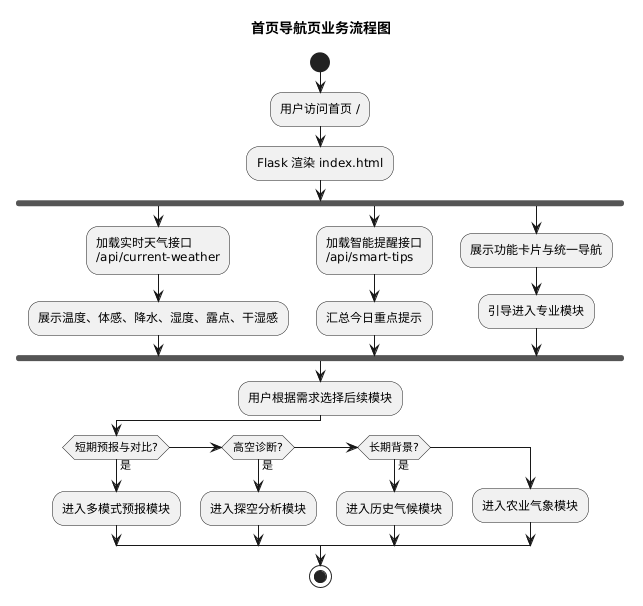
\includegraphics[width=\textwidth]{home_navigation_flow.png}
      {\tiny 首页导航流程}
  \end{columns}
  \note{从日常痛点切入——打开天气App看到"明天25°C"，但背后是哪个预报模式算出来的？有没有系统性偏暖？今年这个温度在历史上算不算异常？杭州还没有这样一个集成的综合平台。}
\end{frame}

% ═══════════════════════════════════════════
% SLIDE 4: 本文工作
% ═══════════════════════════════════════════
\begin{frame}{本文主要工作}
  \begin{columns}[T]
    \column{0.62\textwidth}
      \begin{enumerate}
        \item 构建基于 Flask 的综合气象信息服务平台\\{\small（五层架构，统一站点/时次口径）}
        \item 集成 ECMWF/GFS/ICON 多模式预报\\{\small（72h 精细化 + 多模式对比）}
        \item 实现探空专业诊断模块\\{\small（Skew-T 图 + CAPE/CIN 稳定度参数 + 风险解读）}
        \item 设计 EW 指数代表事件识别方法\\{\small（历史同日比较 + 过程去重 + 季节分组）}
        \item 建立 ML 误差校正链路\\{\small（温度 MAE $\downarrow$22.2\%，风速 $\downarrow$40.8\%）}
        \item 延伸农业气象行业服务\\{\small（5 种作物，积温/适宜度/风险预警/AI 建议）}
      \end{enumerate}
    \column{0.33\textwidth}
      \centering
      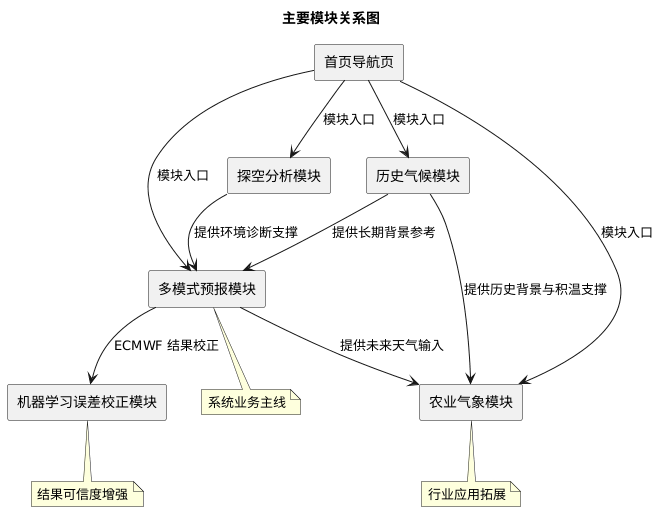
\includegraphics[width=\textwidth]{module_relationship.png}
      {\tiny 模块协同关系}
  \end{columns}
  \note{六项工作快速过。重点不是念，而是让老师先知道系统涵盖哪些方面。后面每个点都会展开。}
\end{frame}

% ═══════════════════════════════════════════
% SLIDE 5: 系统总体架构
% ═══════════════════════════════════════════
\section{系统总体设计}
\begin{frame}{系统总体架构：五层设计}
  \centering
  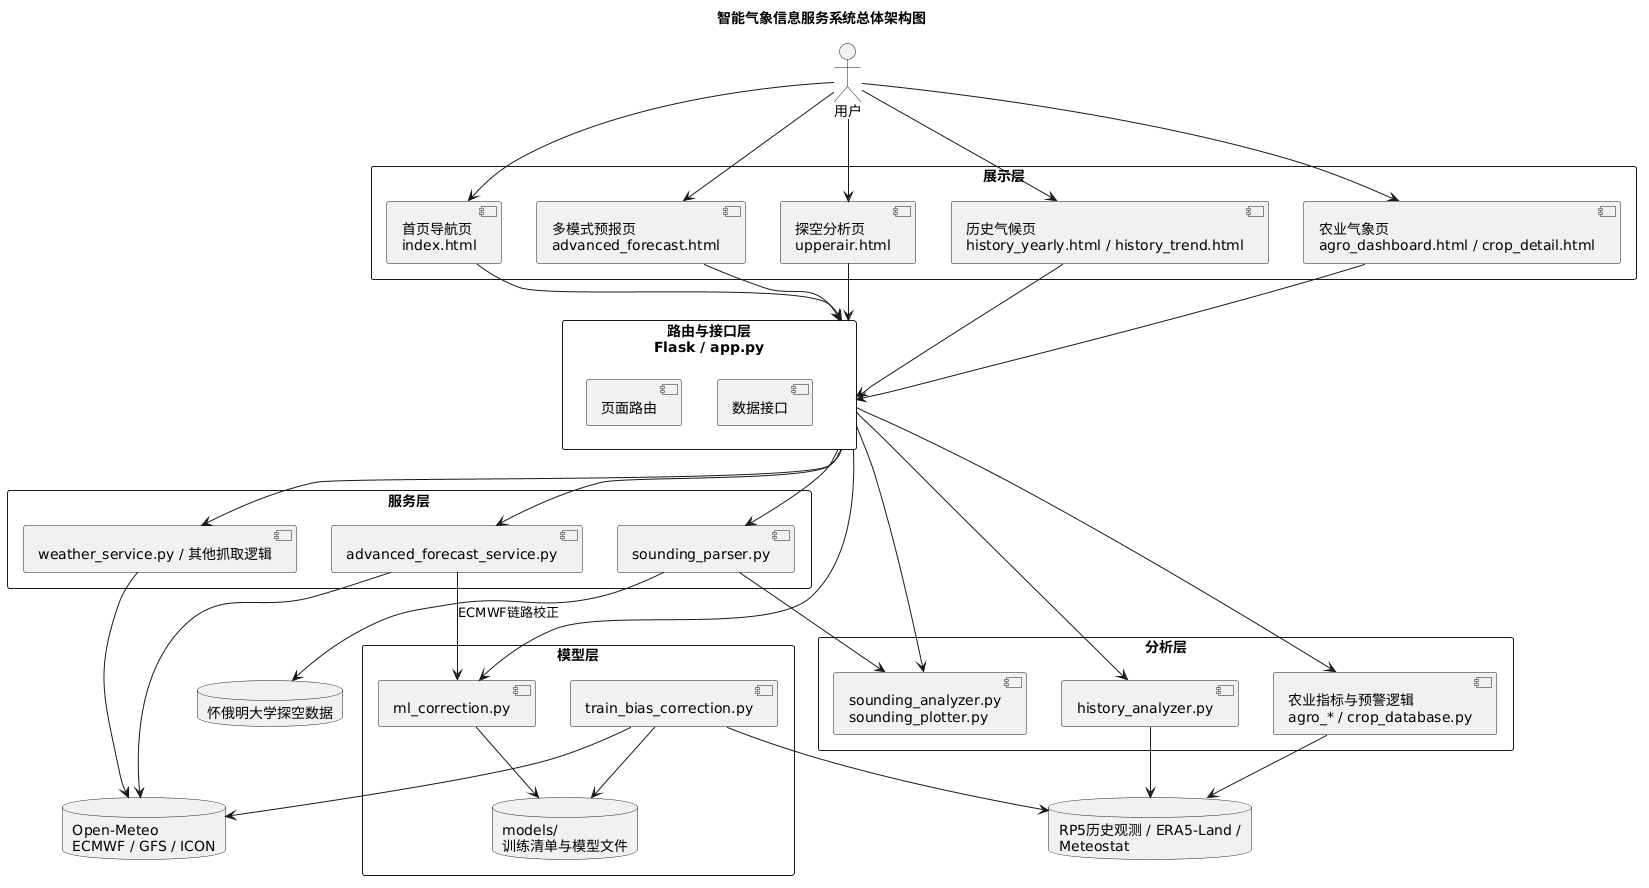
\includegraphics[width=0.92\textwidth]{system_architecture.png}
  \vspace{2mm}
  \begin{columns}[T]
    \column{0.18\textwidth}
      \centering\small\textcolor{primary}{展示层}\\\tiny HTML/JS/CSS
    \column{0.18\textwidth}
      \centering\small\textcolor{primary}{路由接口层}\\\tiny Flask app.py
    \column{0.18\textwidth}
      \centering\small\textcolor{primary}{服务层}\\\tiny 数据获取与缓存
    \column{0.18\textwidth}
      \centering\small\textcolor{primary}{分析层}\\\tiny 气象计算与统计
    \column{0.18\textwidth}
      \centering\small\textcolor{primary}{模型层}\\\tiny ML 误差校正
  \end{columns}
  \vspace{2mm}
  {\small 所有模块统一锚定 \textbf{杭州 58457 站 / 馒头山} 口径}
  \note{这是系统最核心的架构图。分层后各模块独立开发但通过统一路由和站点口径协同。以后增加新站点、新作物、新模型不需要推倒重来。}
\end{frame}

% ═══════════════════════════════════════════
% SLIDE 6: 数据流
% ═══════════════════════════════════════════
\begin{frame}{核心数据流：获取 → 清洗 → 分析 → 展示}
  \begin{columns}[T]
    \column{0.45\textwidth}
      \centering
      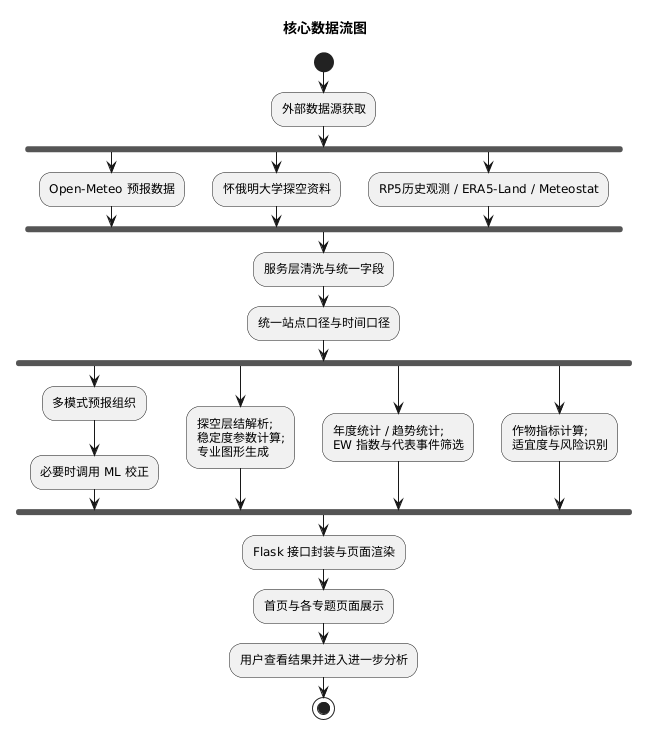
\includegraphics[width=\textwidth]{data_flow.png}
    \column{0.50\textwidth}
      \begin{itemize}
        \item \textbf{外部获取}：Open-Meteo / 怀俄明大学 / 历史站点数据
        \item \textbf{清洗统一}：站点→杭州 58457，时间→UTC 标准时次
        \item \textbf{分析计算}：探空参数 / 历史统计 / 农业指标
        \item \textbf{页面展示}：Plotly.js / Chart.js / Matplotlib+MetPy
      \end{itemize}
      \vspace{4mm}
      {\small\color{highlight}\textbf{关键设计：}训练与运行使用同一站点口径\\→ ML 误差校正结果可解释、可追溯}
  \end{columns}
  \note{数据从外部到用户屏幕的完整路径。强调统一口径——训练用杭州58457、运行也用58457，这是后面ML校正可信度的基础。}
\end{frame}

% ═══════════════════════════════════════════
% SLIDE 7: 首页展示
% ═══════════════════════════════════════════
\begin{frame}{首页：统一入口 + 实时概览 + 模块分发}
  \centering
  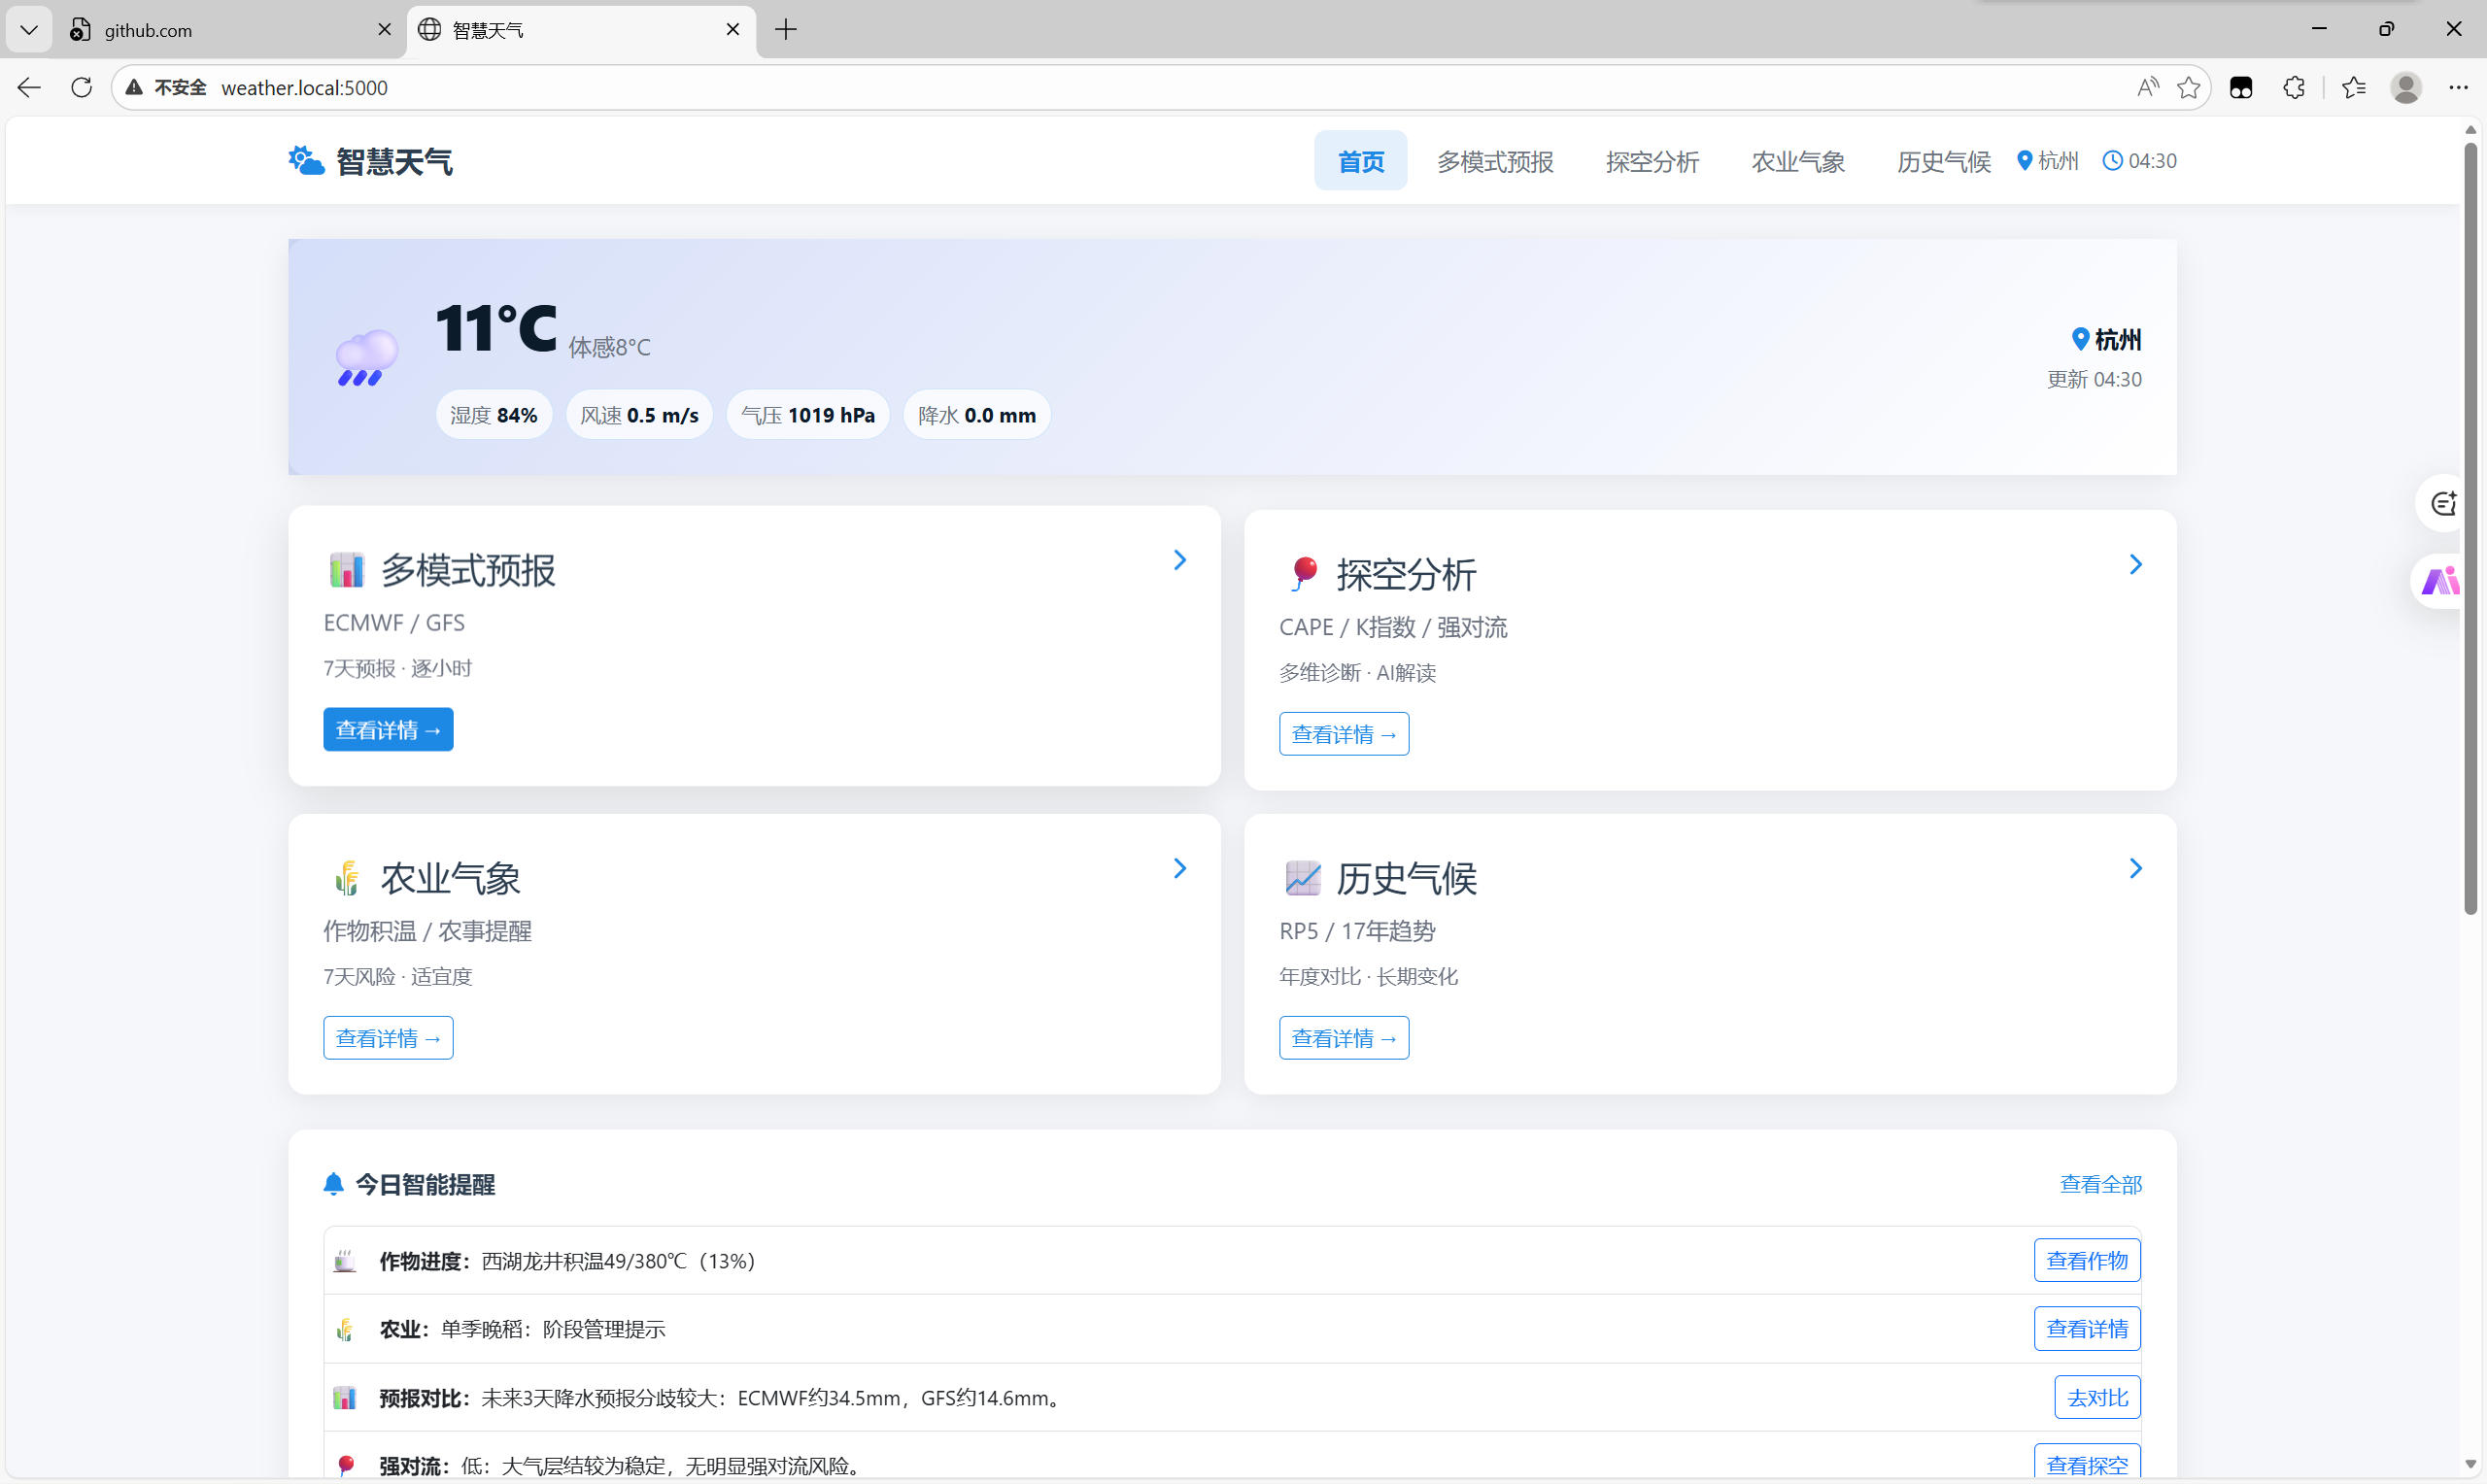
\includegraphics[width=0.88\textwidth]{home1.png}
  \vspace{2mm}
  {\small 顶部：实时天气与体感提示 \quad$\bullet$\quad 中部：五大模块导航卡片 \quad$\bullet$\quad 右侧：智能提醒汇总}
  \note{快速展示首页。首页不只是欢迎页——实时天气、模块入口、智能提醒三位一体。农业预警、预报分歧、探空风险都会在这里汇总显示。}
\end{frame}

% ═══════════════════════════════════════════
% 模块一：多模式预报（Slides 8-10）
% ═══════════════════════════════════════════
\section{多模式预报模块}

\begin{frame}{多模式预报：从"看天气"到"对比分析"}
  \begin{columns}[T]
    \column{0.52\textwidth}
      \begin{itemize}
        \item \textbf{单模式局限}：只给一个结果，无法判断可信度
        \item \textbf{系统思路}：同时展示三种全球模式的预报
          \begin{itemize}
            \item ECMWF（欧洲中期天气预报中心）
            \item GFS（美国全球预报系统）
            \item ICON（德国气象局全球模式）
          \end{itemize}
        \item 72 小时逐小时：温度/降水/湿度/风速变化趋势
      \end{itemize}
    \column{0.43\textwidth}
      \centering
      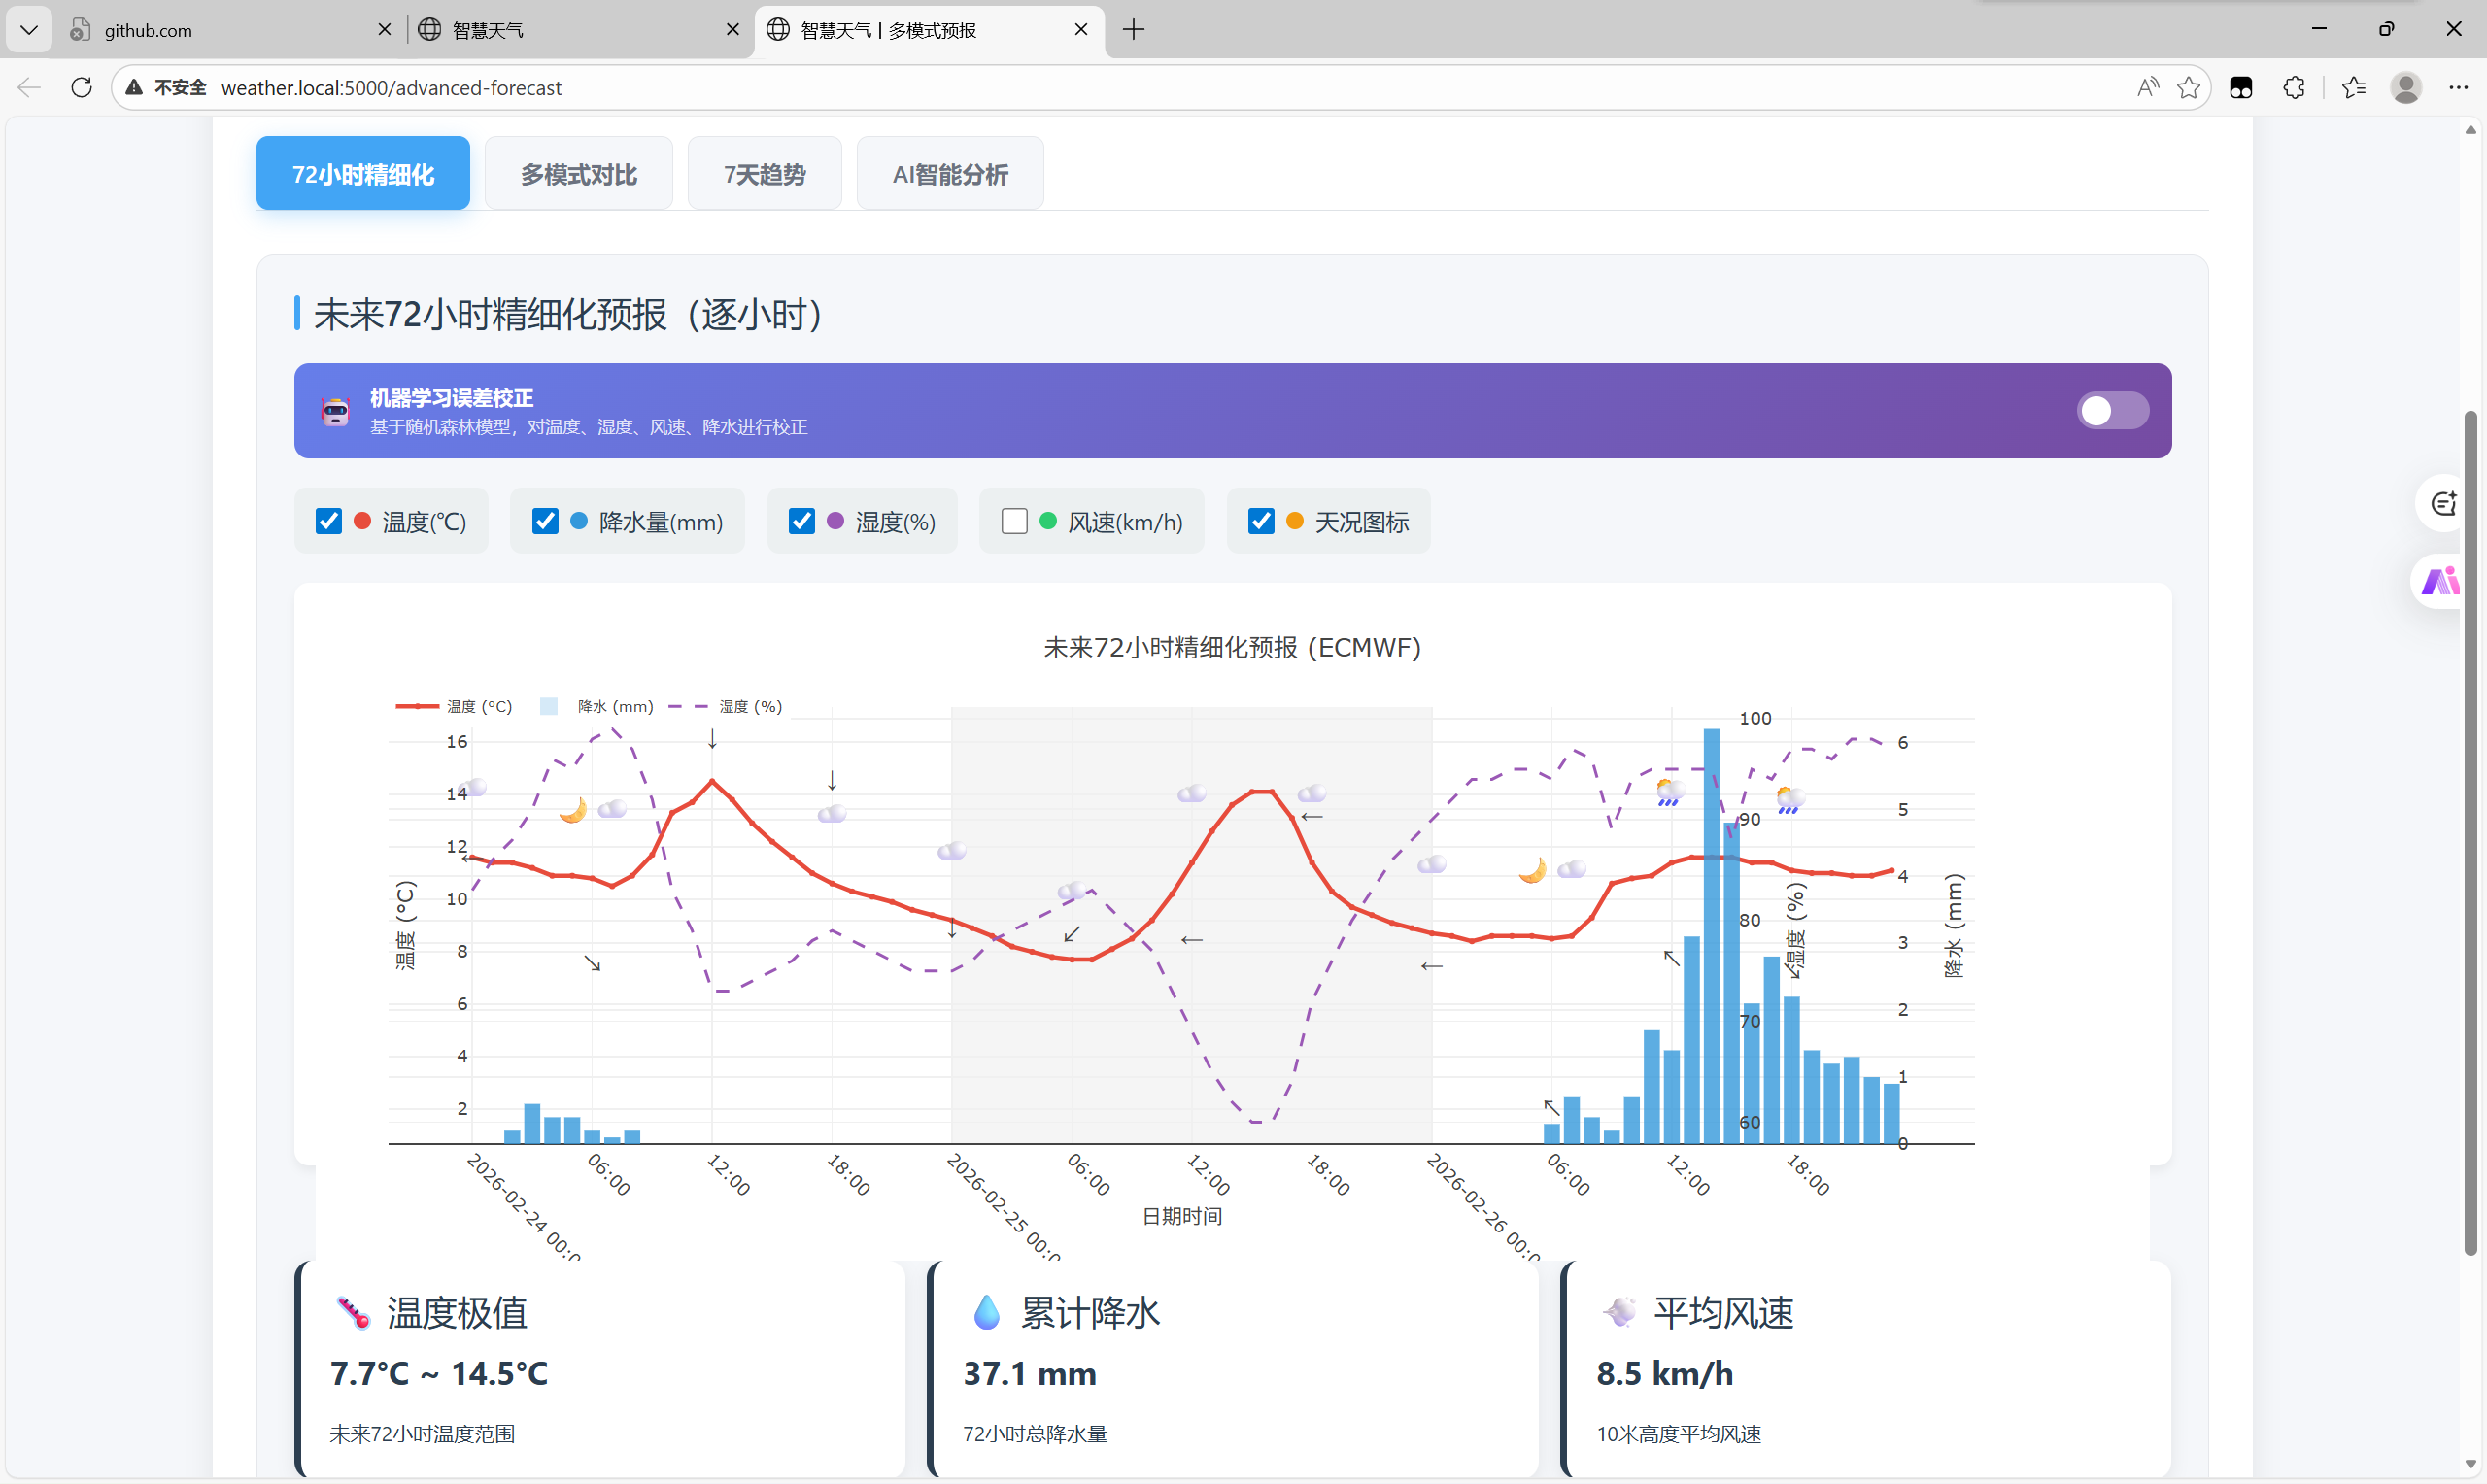
\includegraphics[width=\textwidth]{advanced-forecast1.png}
      {\tiny 72小时精细化预报页面}
  \end{columns}
  \note{建立"为什么需要多模式"的认知——同一时间地点，不同模式结果可能差好几度。只看到一个结果，用户没法判断预报可信度。多模式并列对比就能看出判断是否一致。}
\end{frame}

\begin{frame}{多模式预报：技术实现}
  \begin{columns}[T]
    \column{0.42\textwidth}
      \centering
      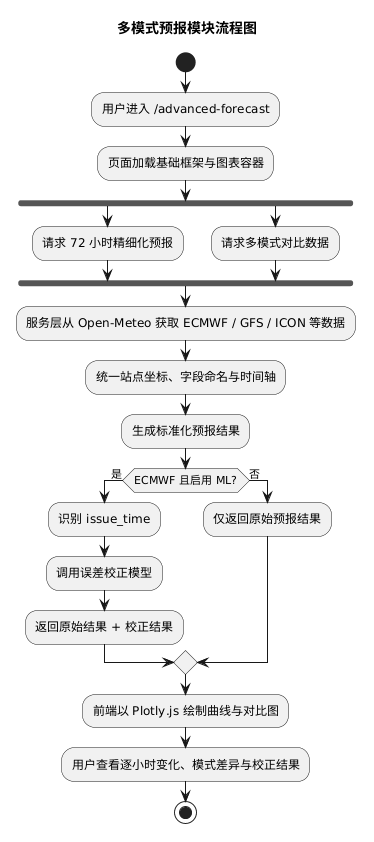
\includegraphics[width=\textwidth]{advanced_forecast_flow.png}
    \column{0.53\textwidth}
      \begin{itemize}
        \item \textbf{数据获取}：Open-Meteo API 统一接口\\{\small（一次调用获取三种模式数据）}
        \item \textbf{并行请求}：三模式同时获取，避免串行等待
        \item \textbf{前端展示}：Plotly.js 交互曲线\\{\small（缩放、悬停查看具体数值）}
        \item \textbf{异步加载}：页面先渲染框架，数据后台填充
        \item \textbf{短时缓存}：减少重复请求，保证时效性
      \end{itemize}
  \end{columns}
  \note{四个技术关键点——统一API接口、并行请求、Plotly.js交互图、异步加载。并行请求确保ECMWF慢不会把GFS也卡住。异步加载让页面先出来，数据后面填上。}
\end{frame}

\begin{frame}{多模式预报：ML 校正与模型对比}
  \begin{columns}[T]
    \column{0.48\textwidth}
      \centering
      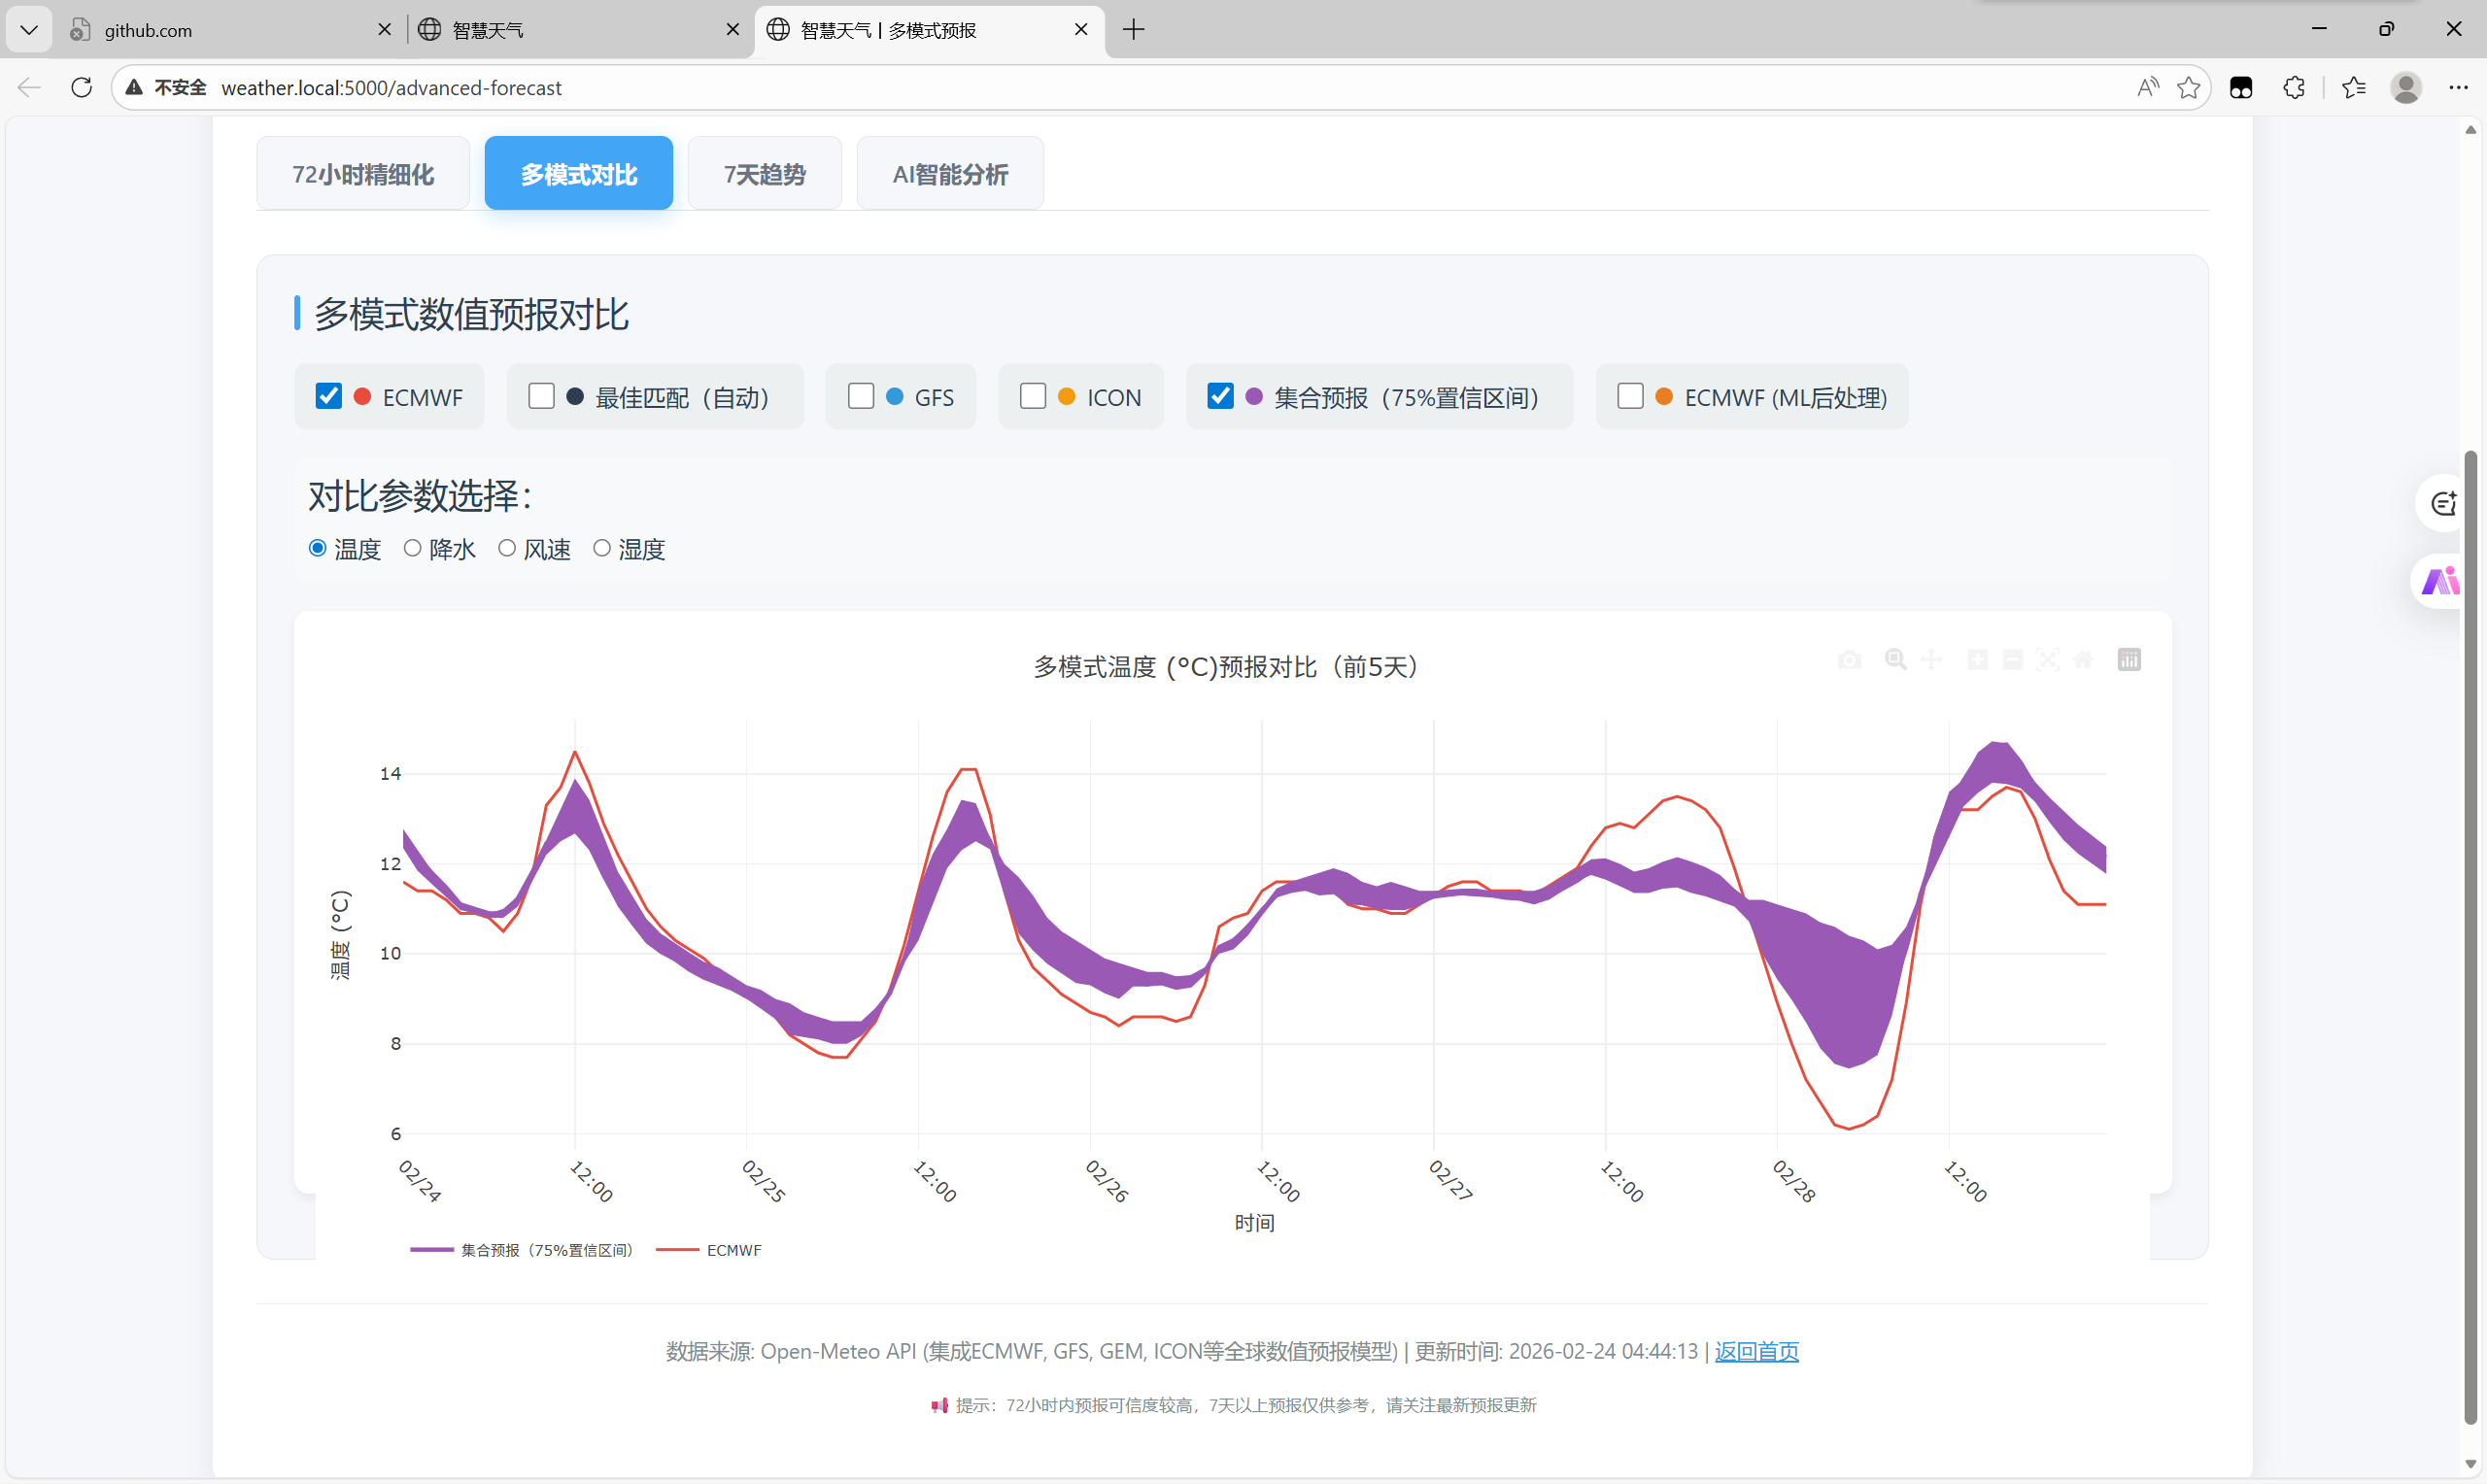
\includegraphics[width=\textwidth]{advanced-forecast2.png}
      {\tiny 多模式同轴对比}
    \column{0.48\textwidth}
      \centering
      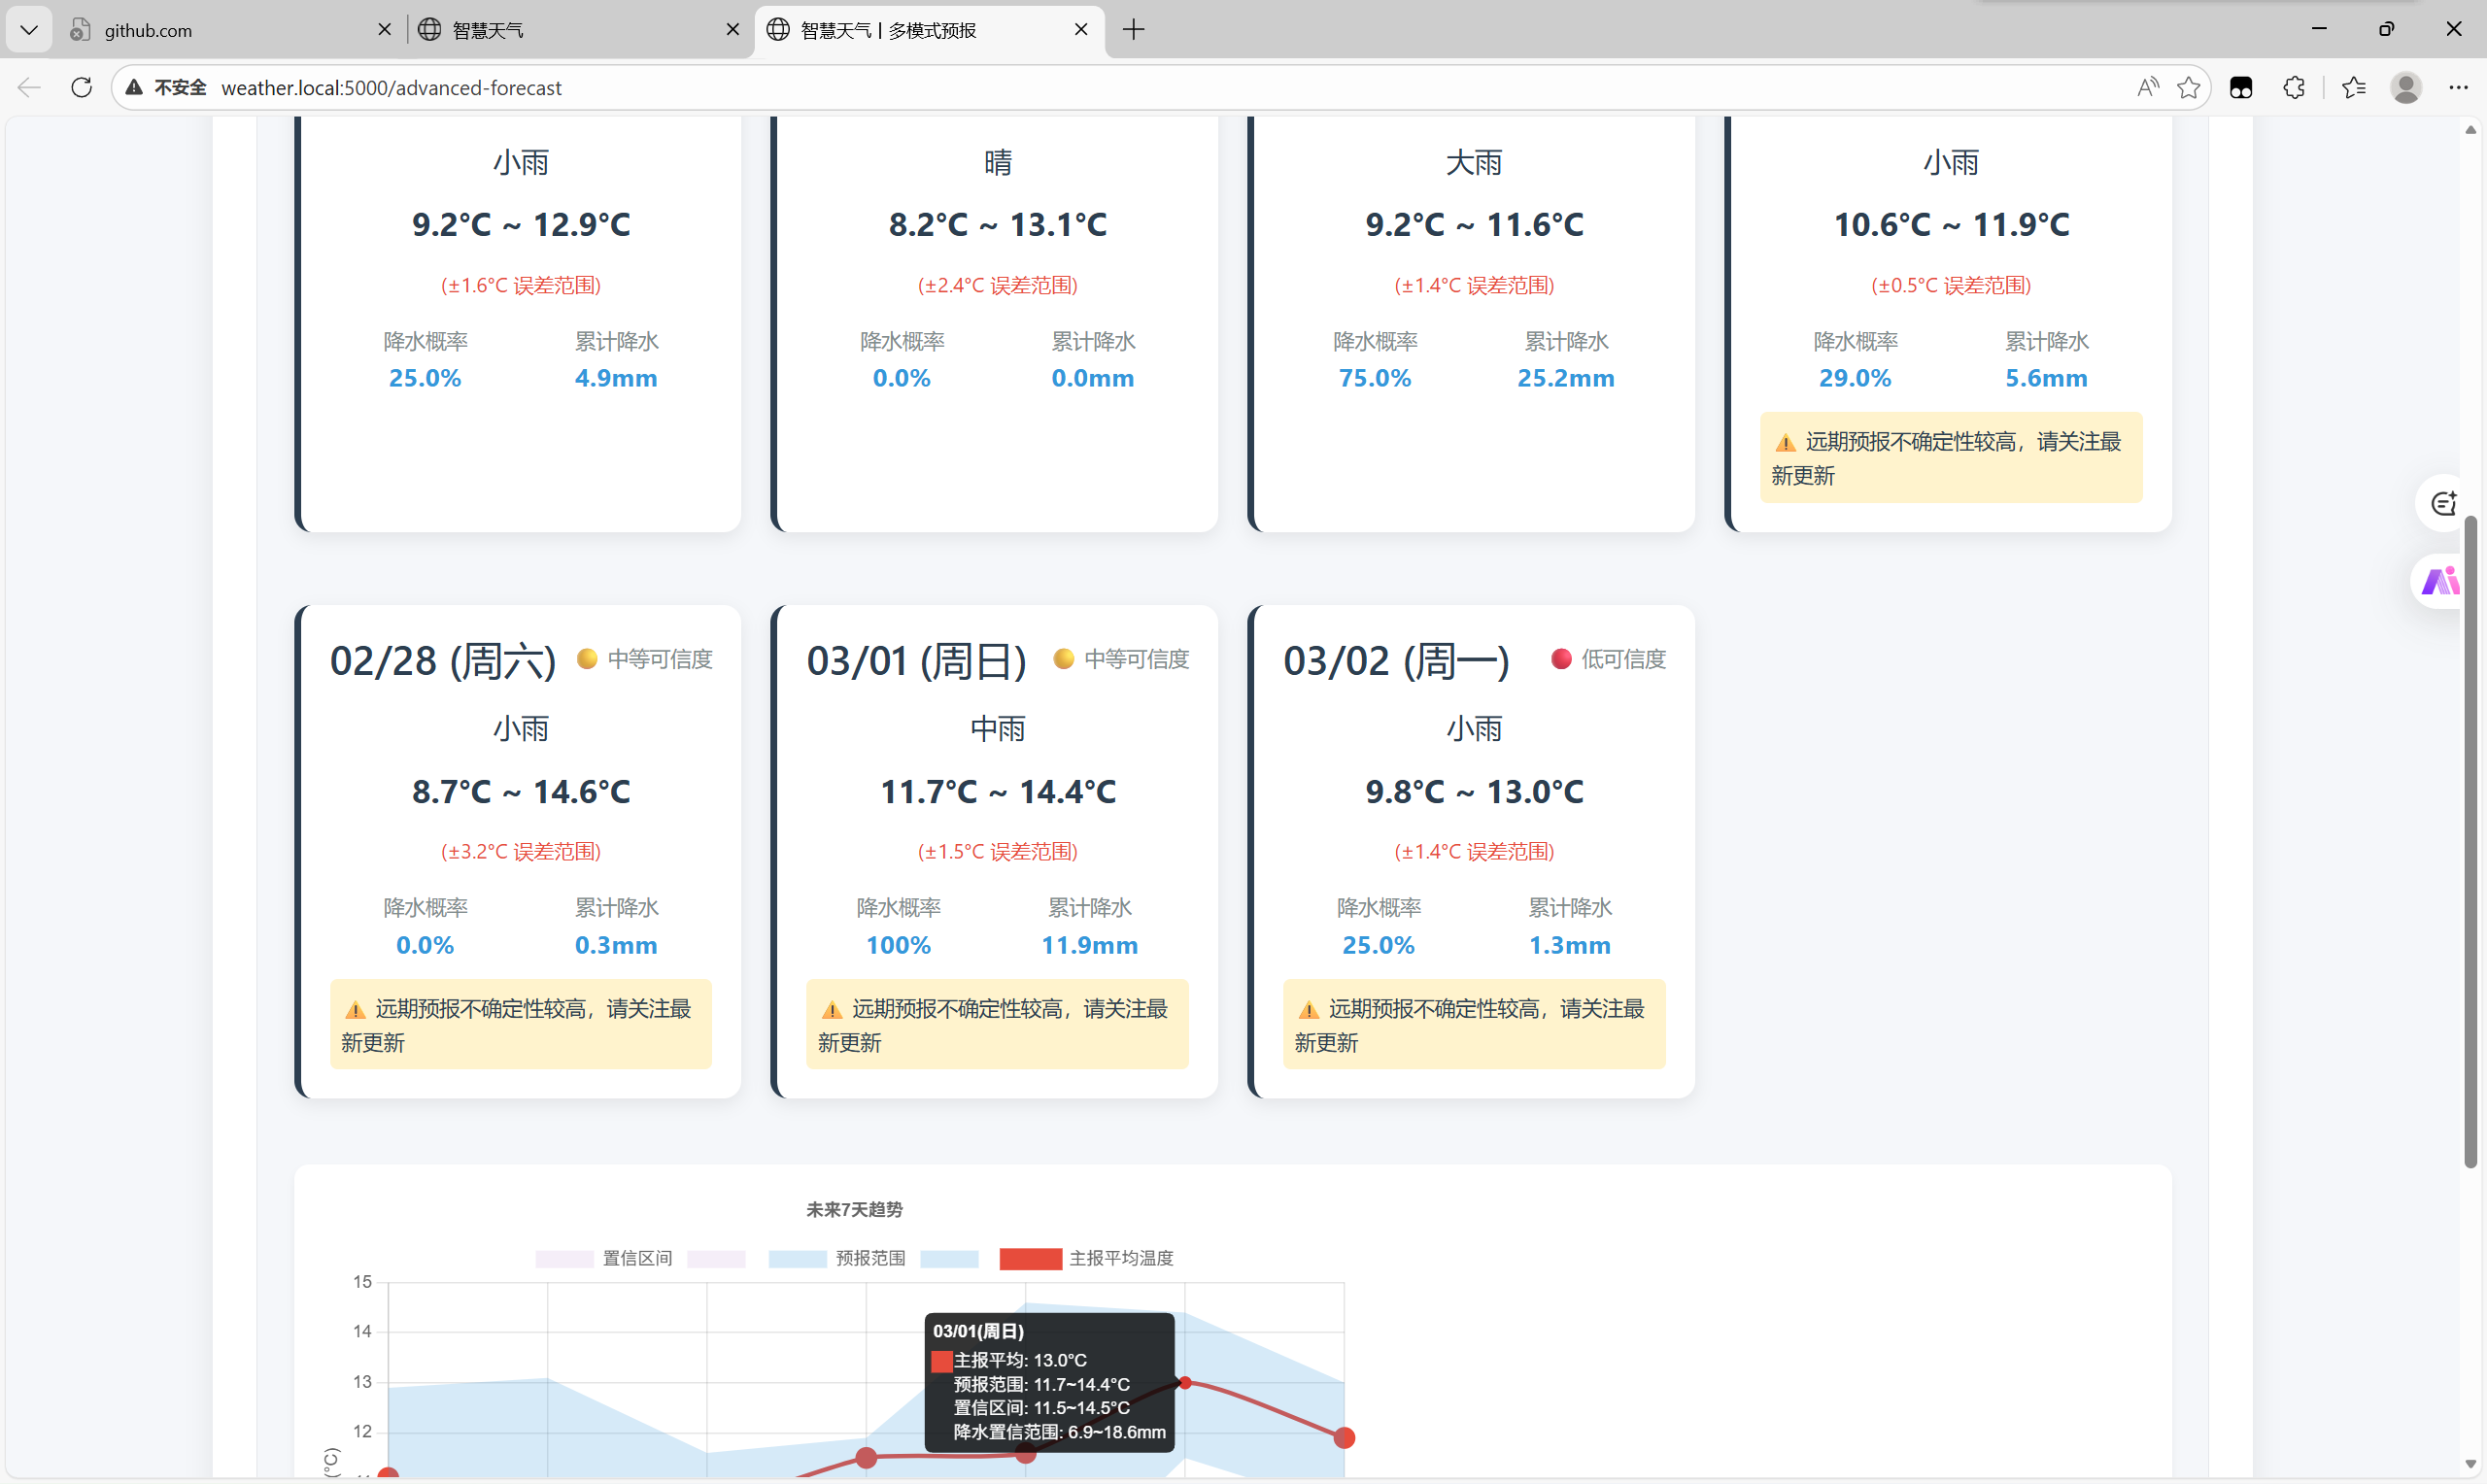
\includegraphics[width=\textwidth]{advanced-forecast3.png}
      {\tiny ML 校正结果（温度曲线）}
  \end{columns}
  \vspace{2mm}
  \begin{itemize}
    \item 多模式同轴对比：ECMWF / GFS / ICON 在同一图上叠加
    \item ML 校正仅对 ECMWF 启用（保持训练/运行口径一致）
    \item 一键切换原始/校正结果，模型异常时自动回退
  \end{itemize}
  \note{左边多模式对比——三条不同颜色曲线代表三个模式，对同一场降温的强度和时间的判断差异一目了然。右边ML校正效果——原始ECMWF和校正后曲线叠在一起，修正幅度清晰可见。}
\end{frame}

% ═══════════════════════════════════════════
% 模块二：探空分析（Slides 11-13）
% ═══════════════════════════════════════════
\section{探空分析模块}

\begin{frame}{探空分析：当"明天有雨"不够时}
  \begin{columns}[T]
    \column{0.42\textwidth}
      \centering
      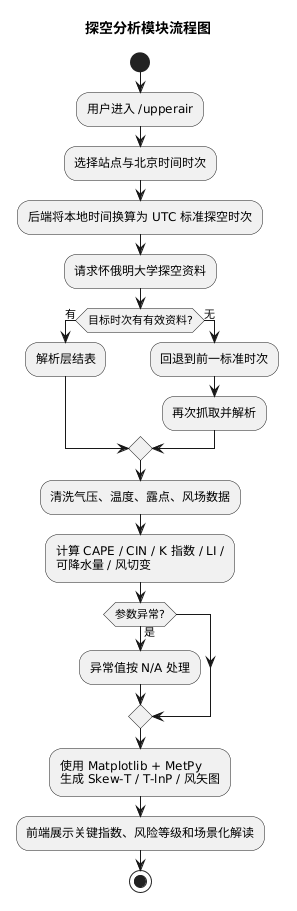
\includegraphics[width=\textwidth]{upperair_flow.png}
    \column{0.53\textwidth}
      \begin{itemize}
        \item \textbf{地面预报}回答"未来怎么样"\\\textbf{探空分析}回答"大气具备什么条件"
        \item 数据来源：怀俄明大学全球探空资料库\\{\small（杭州站 58457，每日 00Z/12Z）}
        \item 北京时间输入 → 后端自动 UTC 转换
        \item 当前时次无数据 → 自动回退前一标准时次
        \item 场景：同样是"明天有雨"——\\{\small 探空判断是普通降雨还是强对流暴雨}
      \end{itemize}
  \end{columns}
  \note{探空是论文最专业的模块。通俗讲就是放探空气球测量不同高度的温度、湿度、风速。如果CAPE值很高说明大气"憋着一股劲"，一旦触发可能雷暴大风。}
\end{frame}

\begin{frame}{Skew-T 图：大气的"X 光片"}
  \begin{columns}[T]
    \column{0.50\textwidth}
      \centering
      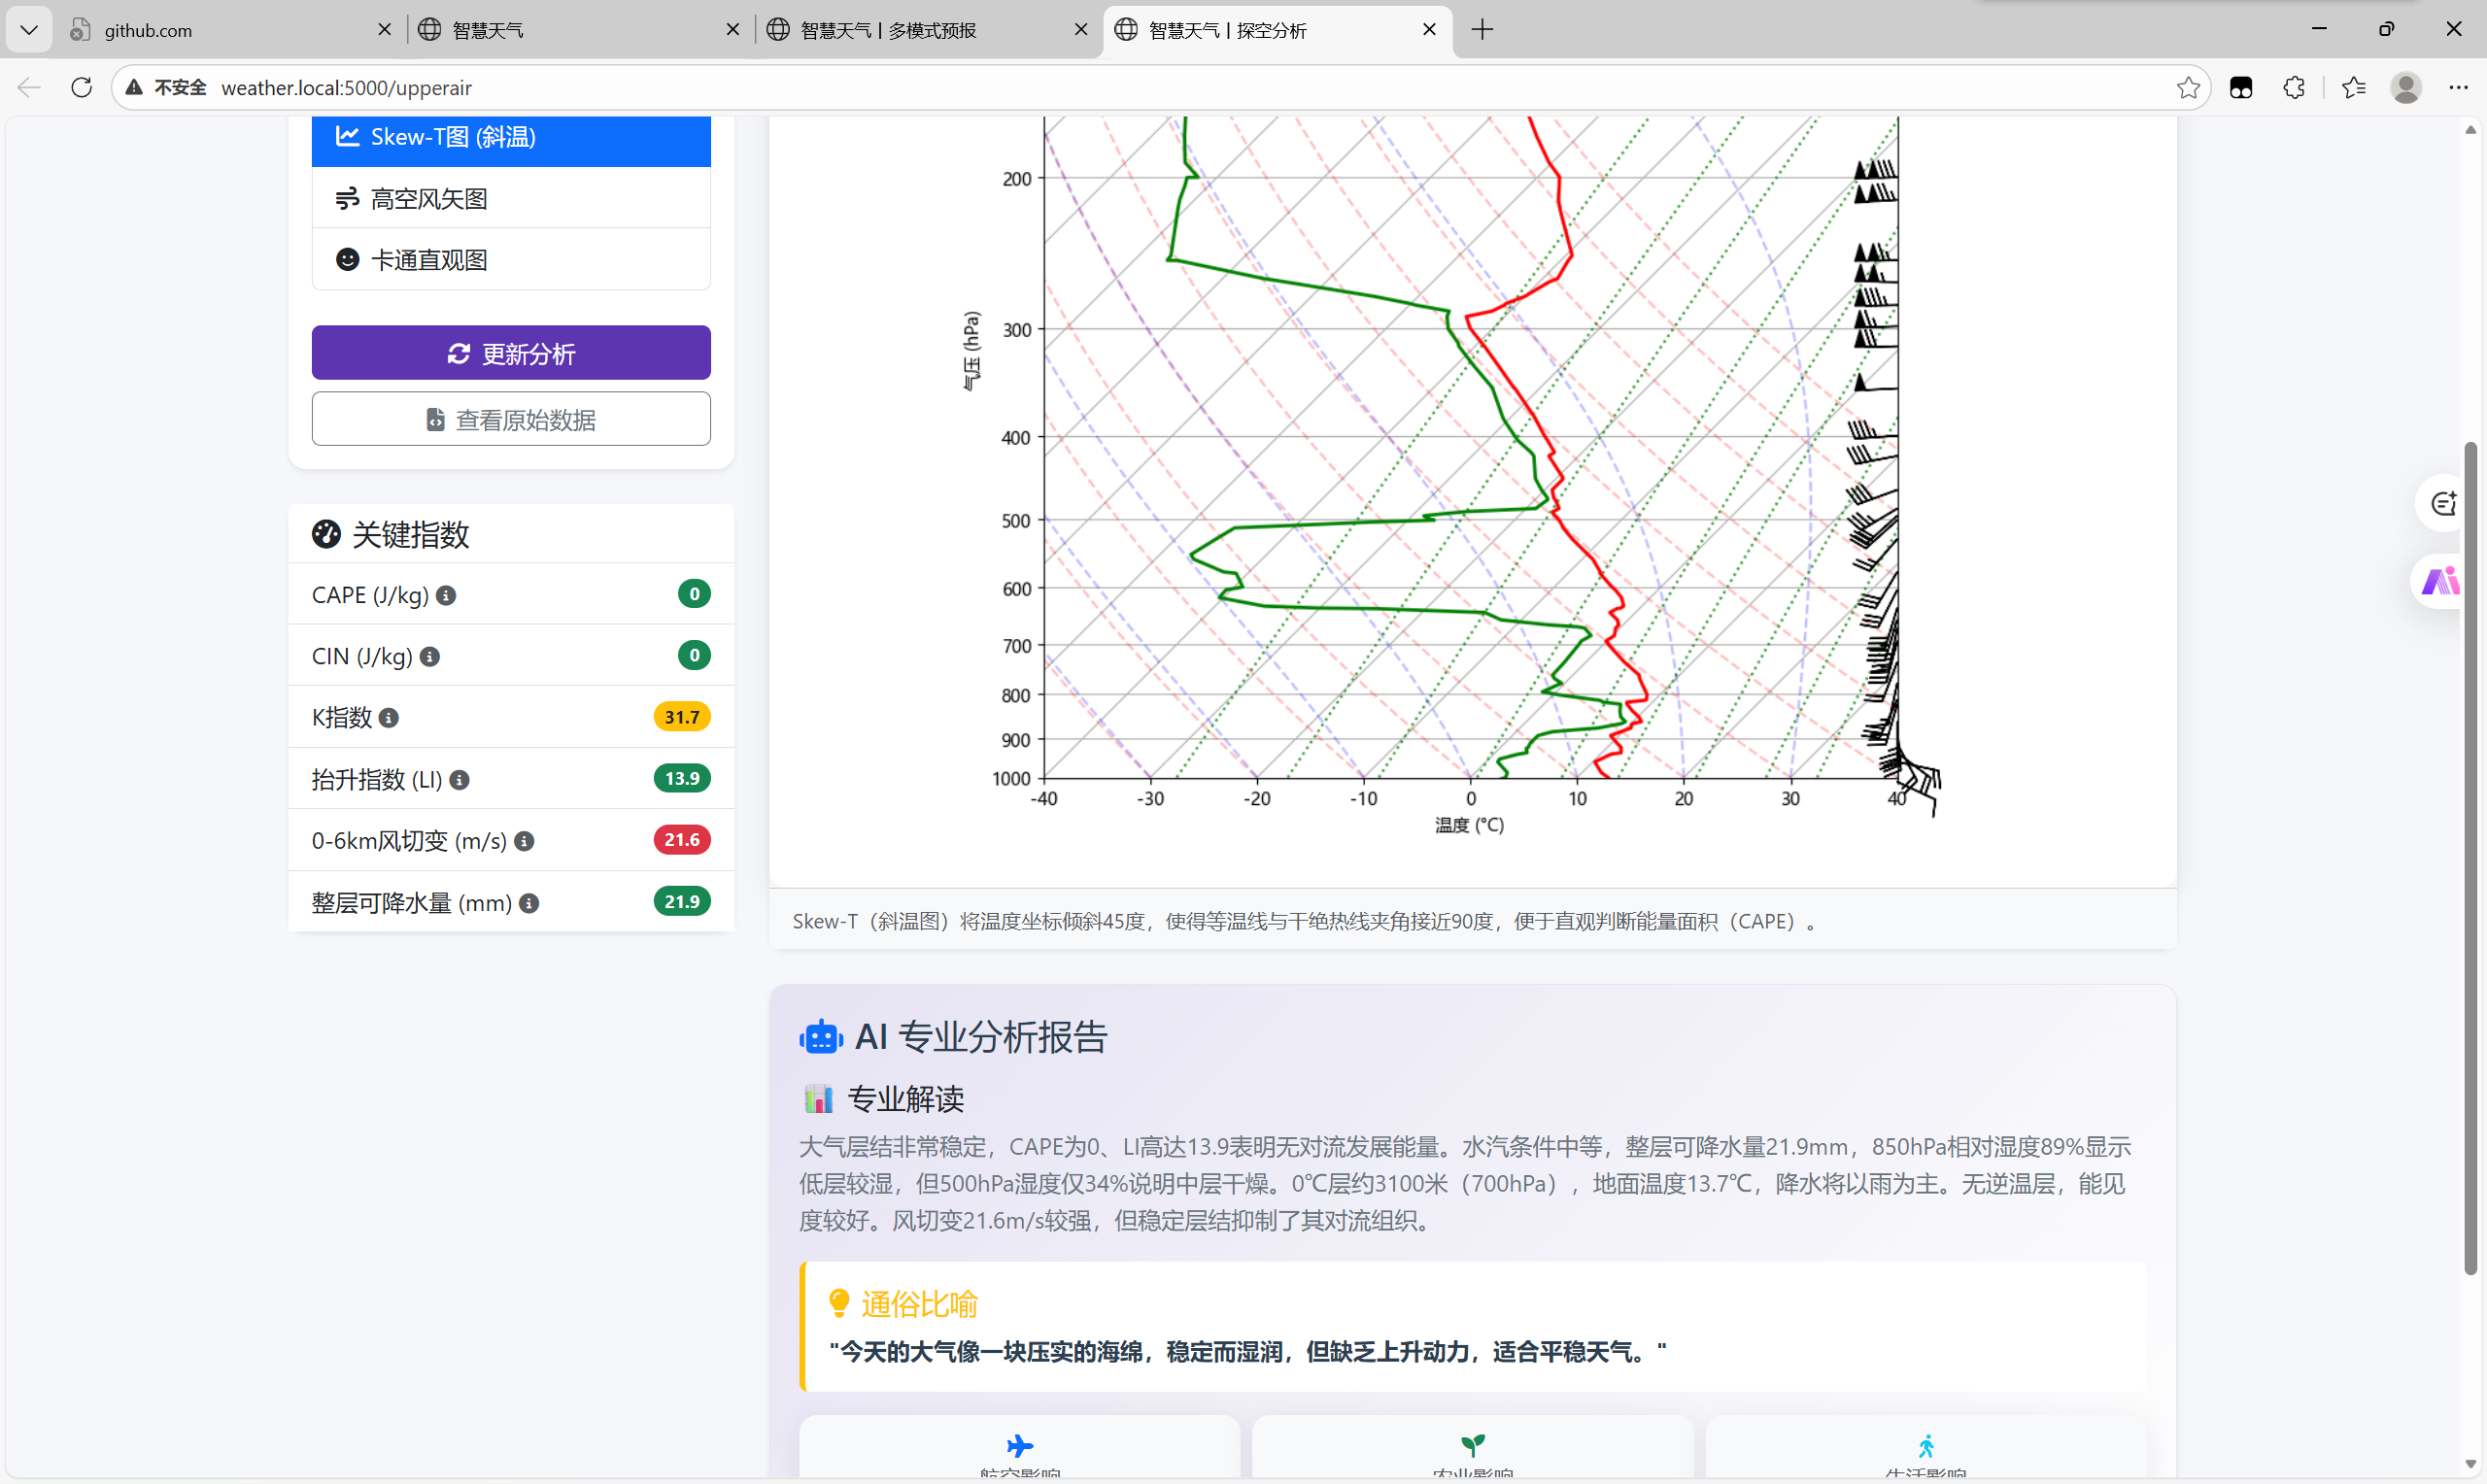
\includegraphics[width=\textwidth]{upperair2.png}
      {\tiny Skew-T 对数压力图（温度/露点廓线 + 风矢量）}
    \column{0.45\textwidth}
      \centering
      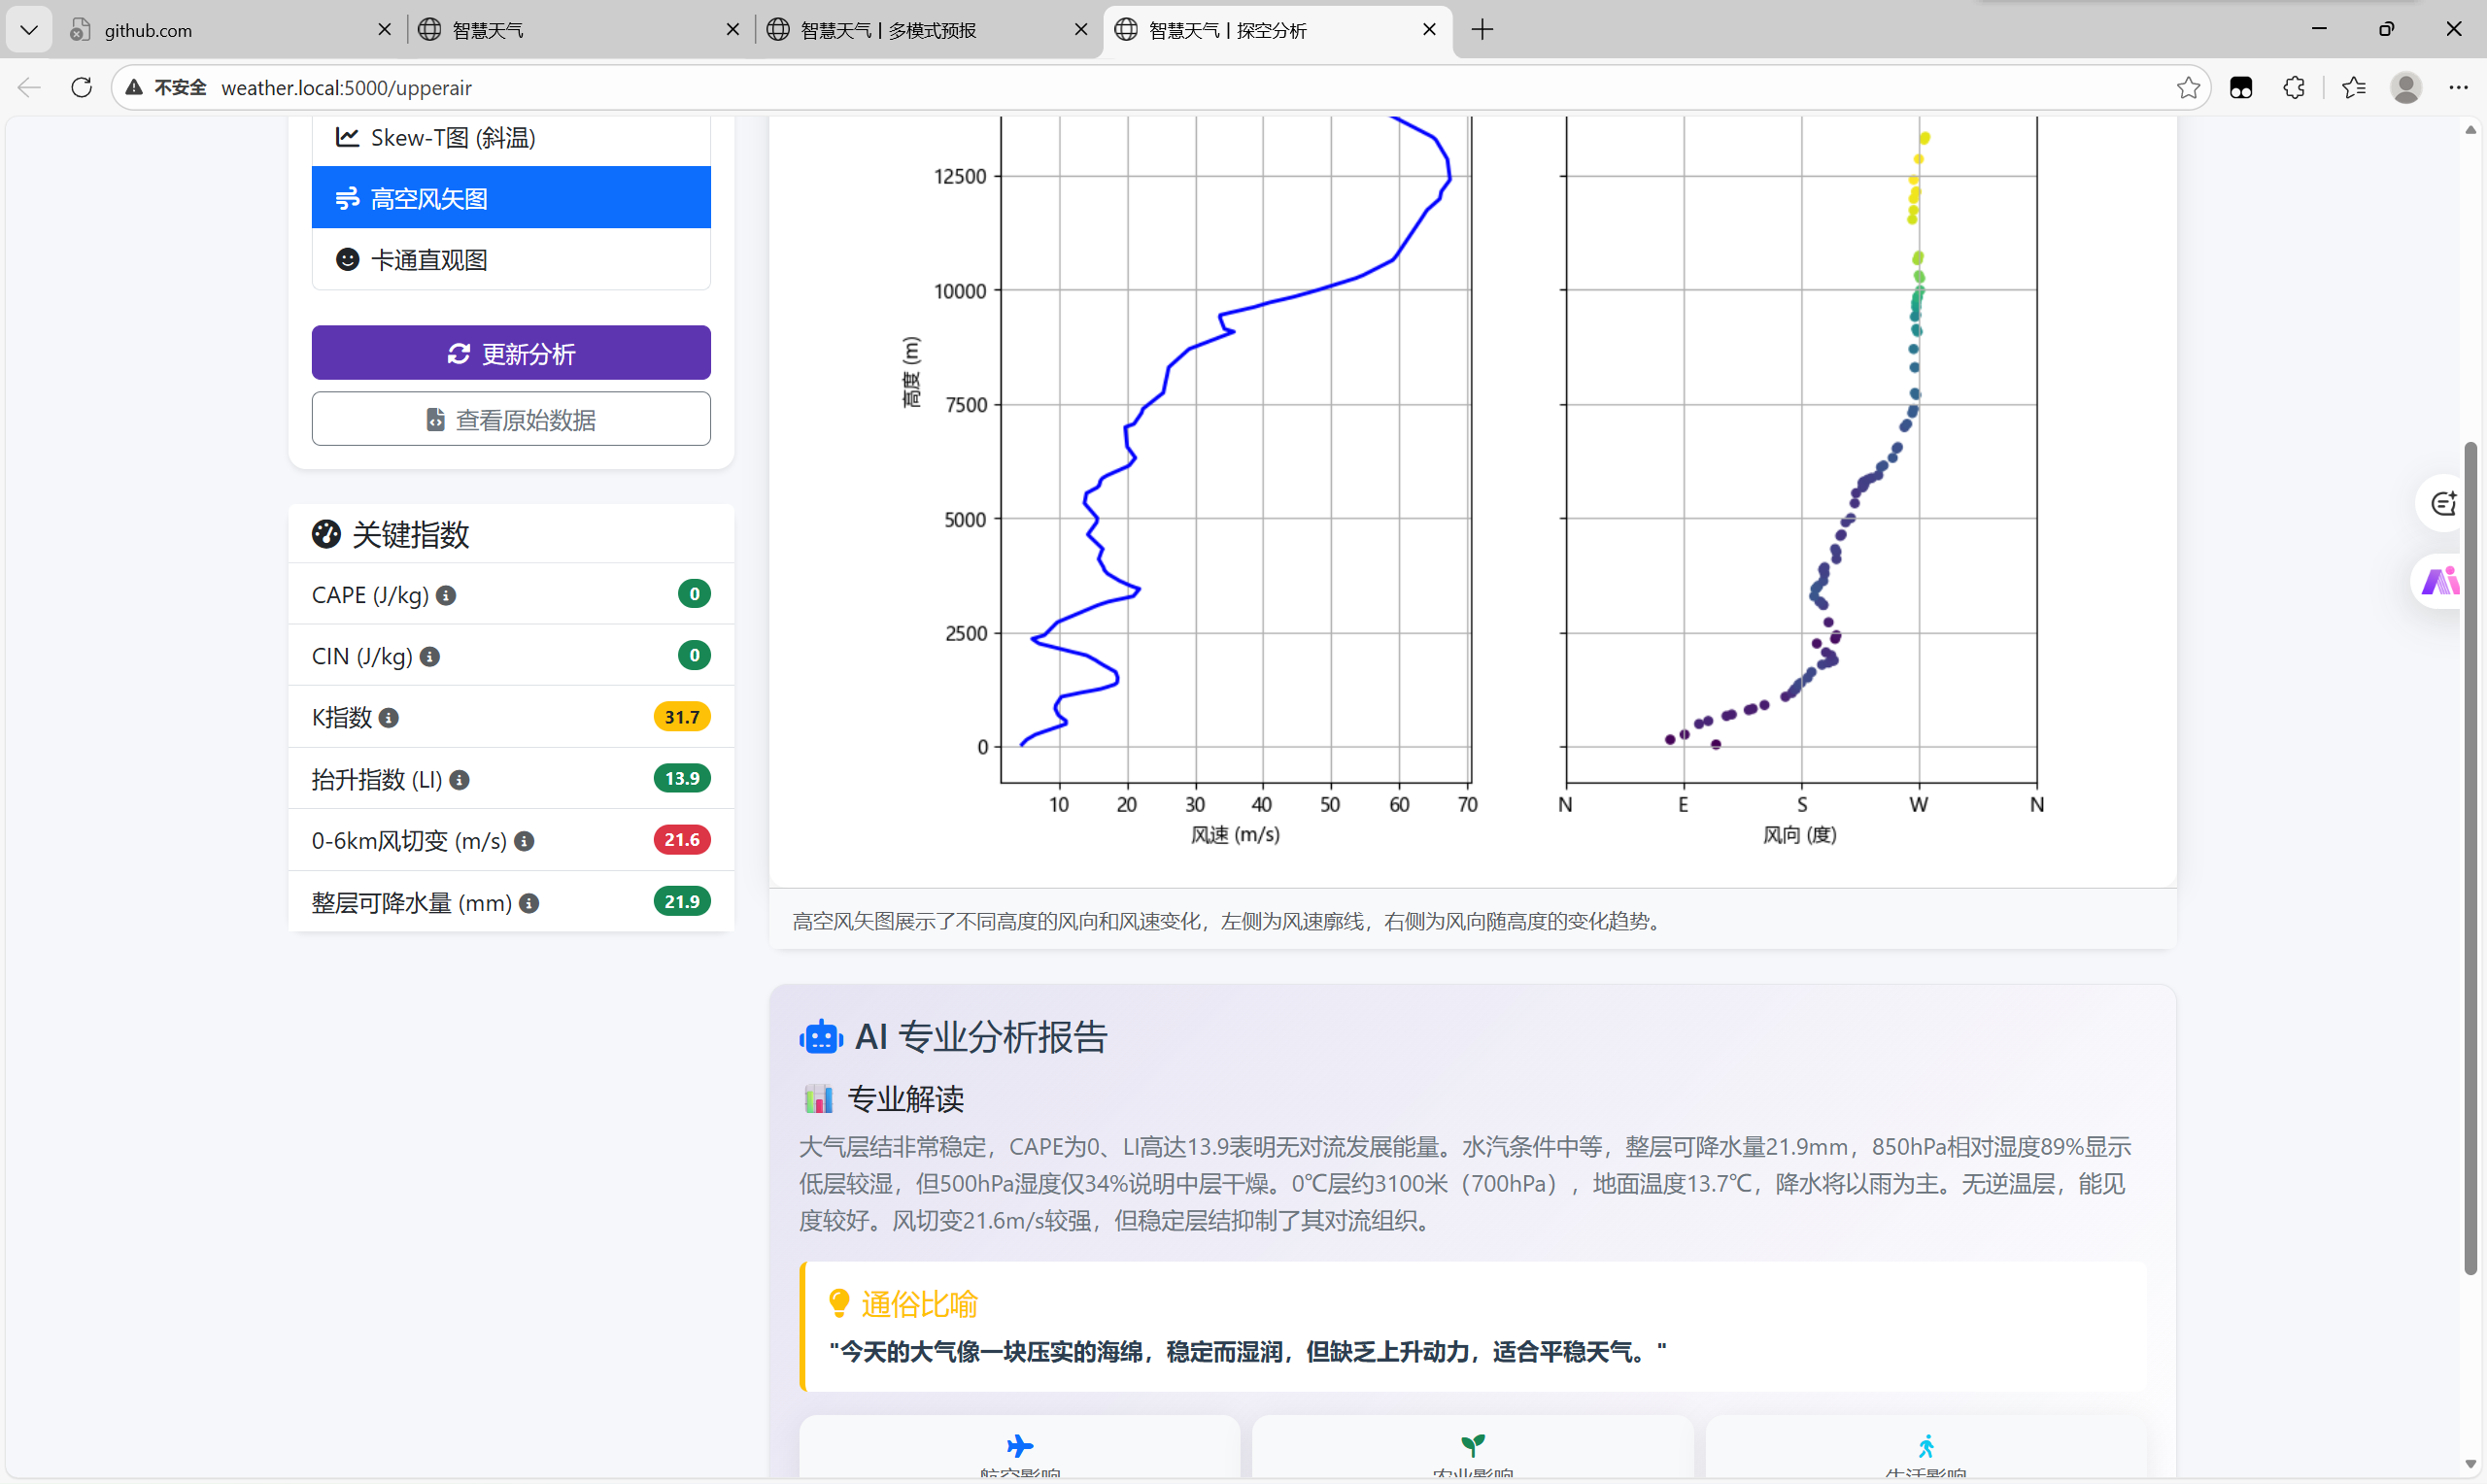
\includegraphics[width=\textwidth]{upperair3.png}
      {\tiny 高空风廓线图}
  \end{columns}
  \vspace{2mm}
  \begin{itemize}
    \item 红色：温度廓线，蓝色：露点廓线 → 越靠近越容易凝结
    \item 紫色阴影 = CAPE（对流有效位能），面积越大对流潜势越强
    \item 系统提供四种图形：Skew-T / T-lnP / 风矢 / 卡通直观图
  \end{itemize}
  \note{指着Skew-T讲——红蓝两条线越近湿度越大。紫色CAPE面积就是积雨云的能量来源。系统提供四种图形，专业用户看Skew-T，非专业看卡通图。}
\end{frame}

\begin{frame}{从专业参数到通俗解读}
  \begin{columns}[T]
    \column{0.48\textwidth}
      \centering
      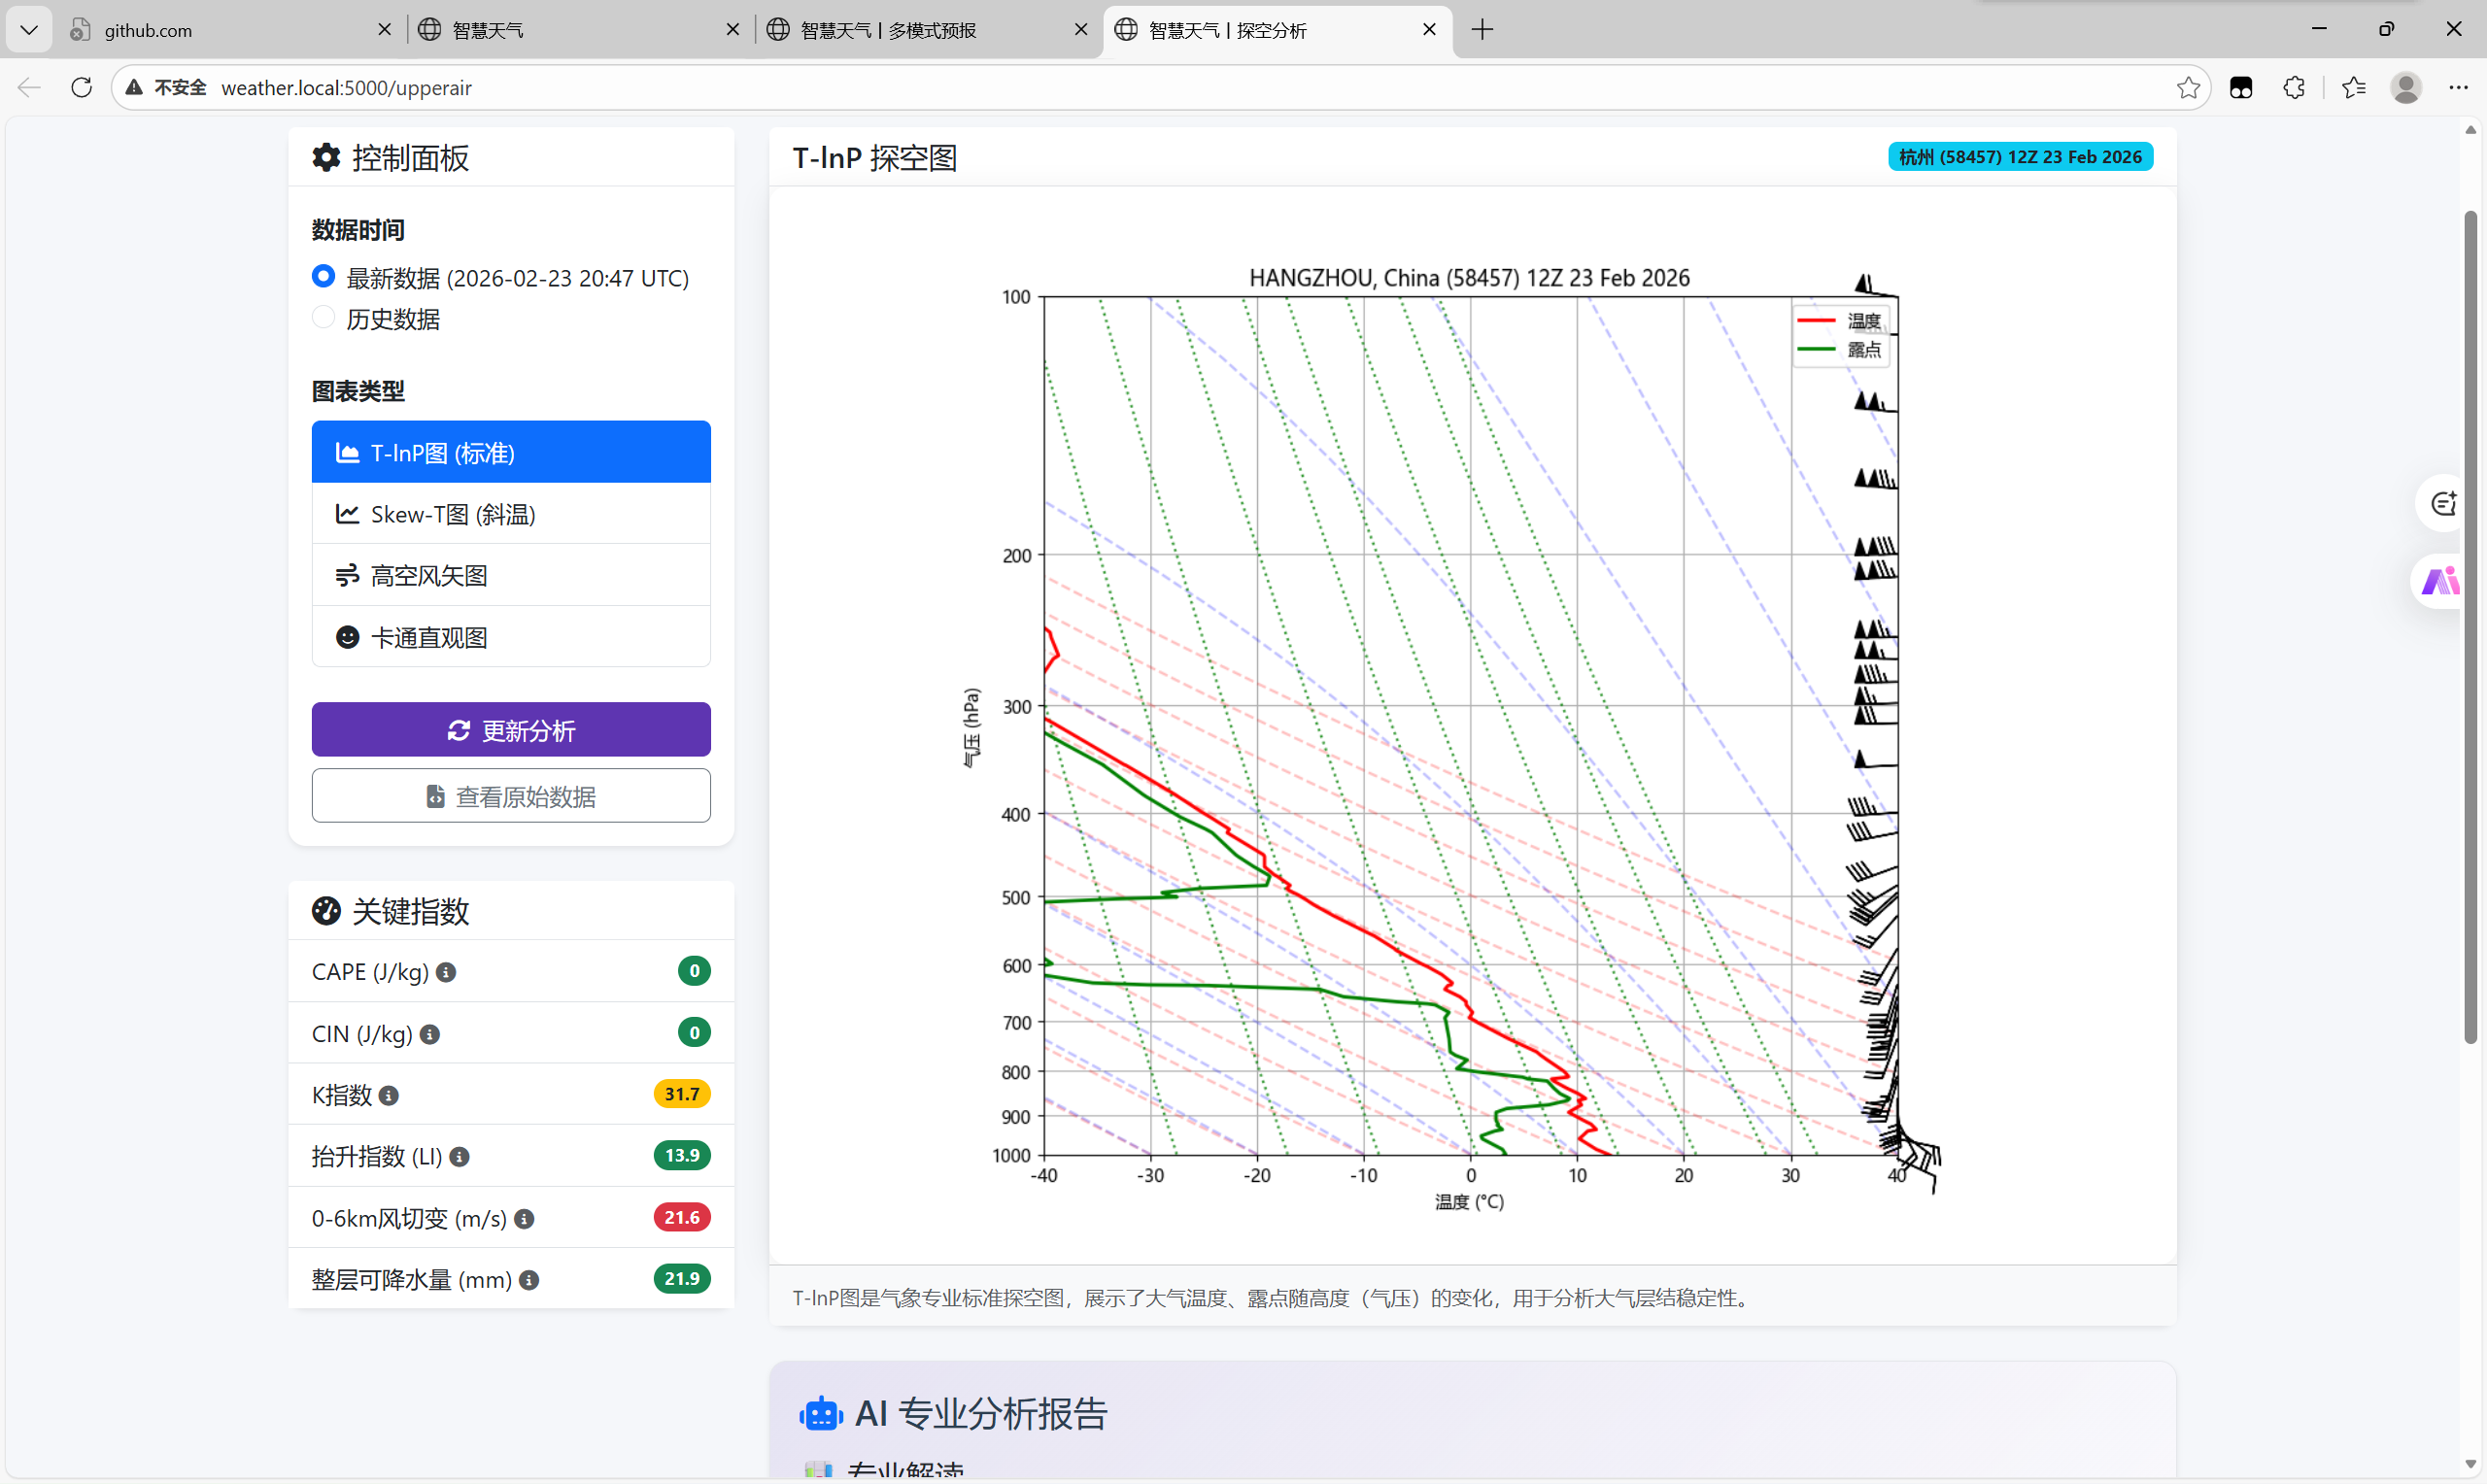
\includegraphics[width=\textwidth]{upperair1.png}
      {\tiny 探空参数面板与风险等级}
    \column{0.48\textwidth}
      \begin{itemize}
        \item \textbf{关键参数}（附中文说明）：
          \begin{itemize}
            \item CAPE 对流有效位能 / CIN 对流抑制
            \item K 指数 / 抬升指数 LI
            \item 0-6km 风切变 / 整层可降水量 PWAT
          \end{itemize}
        \item \textbf{场景化解读}：
          \begin{itemize}
            \item 航空：风切变 / 颠簸风险
            \item 农业：强对流 / 冰雹威胁
            \item 公众：户外活动风险提示
          \end{itemize}
        \item CAPE 为负值 → 统一标注 N/A（防止误解）
      \end{itemize}
  \end{columns}
  \note{参数虽专业但都有中文说明。三视角解读——航空看风切变、农业看强对流、公众看出行。CAPE为负值不显示数字而标N/A，避免给用户一个误导人的负数。}
\end{frame}

% ═══════════════════════════════════════════
% 模块三：历史气候分析（Slides 14-16）
% ═══════════════════════════════════════════
\section{历史气候分析模块}

\begin{frame}{历史气候分析：从单年到多年趋势}
  \begin{columns}[T]
    \column{0.45\textwidth}
      \centering
      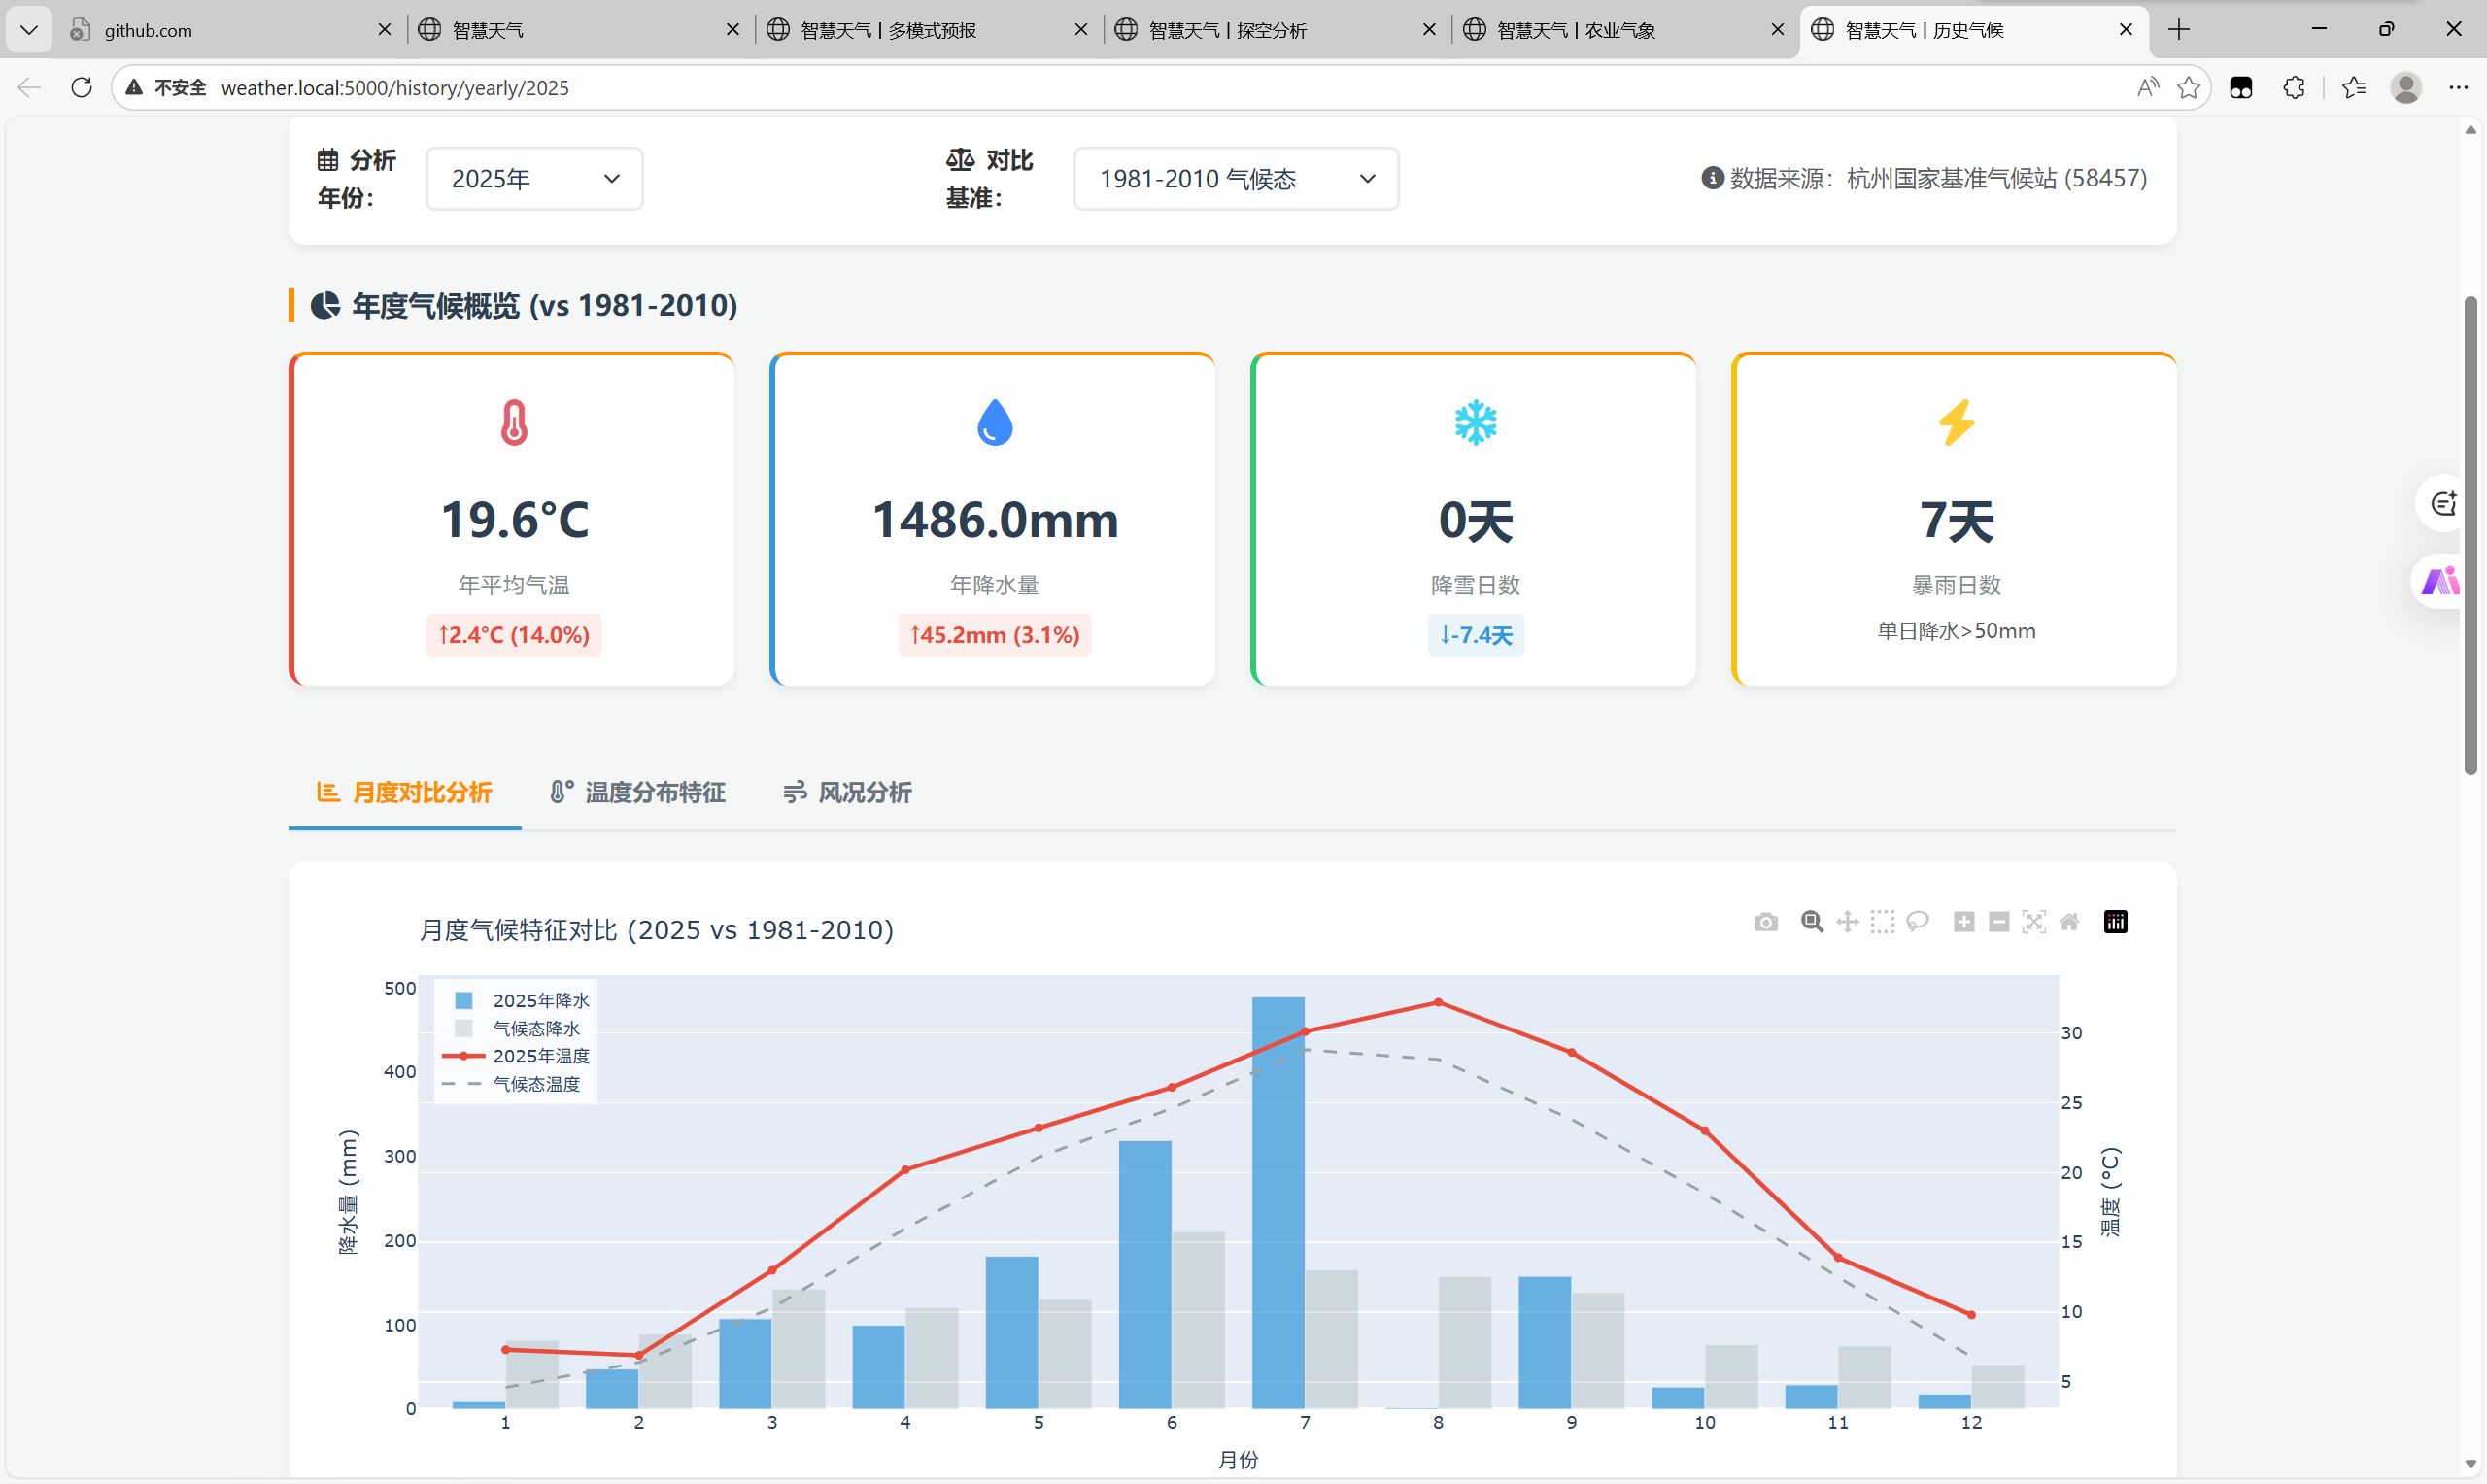
\includegraphics[width=\textwidth]{history.png}
      {\tiny 年度气候概览页}
    \column{0.50\textwidth}
      \begin{itemize}
        \item \textbf{年度统计}：年均温/降水量/雨雪日/极端日数\\{\small 与标准气候态对比，判断偏暖/偏冷/偏湿/偏干}
        \item \textbf{双气候态切换}：1981--2010 / 1991--2020\\{\small 符合气候业务标准}
        \item \textbf{长期趋势}：多年气温/降水/极端频次变化
        \item 可视化：Plotly 月度对比 / 日分布 / 风玫瑰 / 趋势序列
      \end{itemize}
  \end{columns}
  \note{历史气候三件事——单年跟常年比、多年趋势看变化、EW指数挑代表事件。双气候态是业务标准做法，因为不同时期的常年值不一样。}
\end{frame}

\begin{frame}{EW 指数：寻找"真正异常"的天气事件}
  \begin{columns}[T]
    \column{0.42\textwidth}
      \centering
      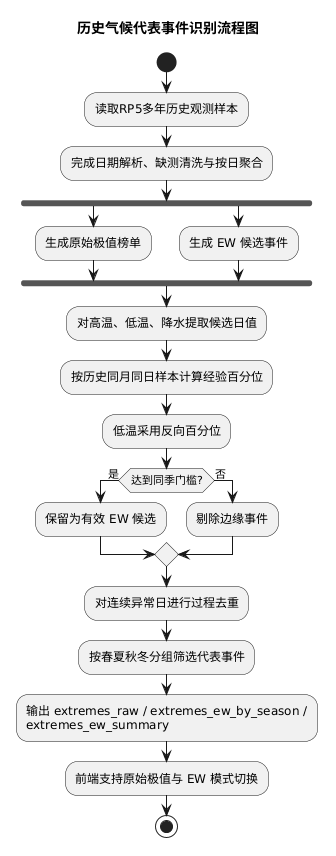
\includegraphics[width=\textwidth]{history_ew_flow.png}
    \column{0.53\textwidth}
      \begin{itemize}
        \item \textbf{问题}：只看绝对值（如"最高温 38°C"）\\$\neq$ 在历史背景中异常
        \item \textbf{EW 指数思路}：同月同日历史样本\\$\rightarrow$ 经验百分位 $\rightarrow$ 异常程度排序
        \item \textbf{设计细节}：
          \begin{itemize}
            \item 低温反向百分位（越冷 $\rightarrow$ 越高极端分）
            \item 同季绝对门槛 + 相邻日过程去重
            \item 四季分组展示（避免某季刷榜）
          \end{itemize}
      \end{itemize}
  \end{columns}
  \note{EW指数最有特色的点。某天38°C看起来很高，但如果过去30年同一天平均37.5°C就不算特别异常。反之32°C但历史同日平均才25°C才是真正的极端。过程去重避免连续5天高温占5条榜单。}
\end{frame}

\begin{frame}{历史气候页：极值榜 + EW 指数双模式}
  \centering
  \begin{columns}[T]
    \column{0.55\textwidth}
      \centering
      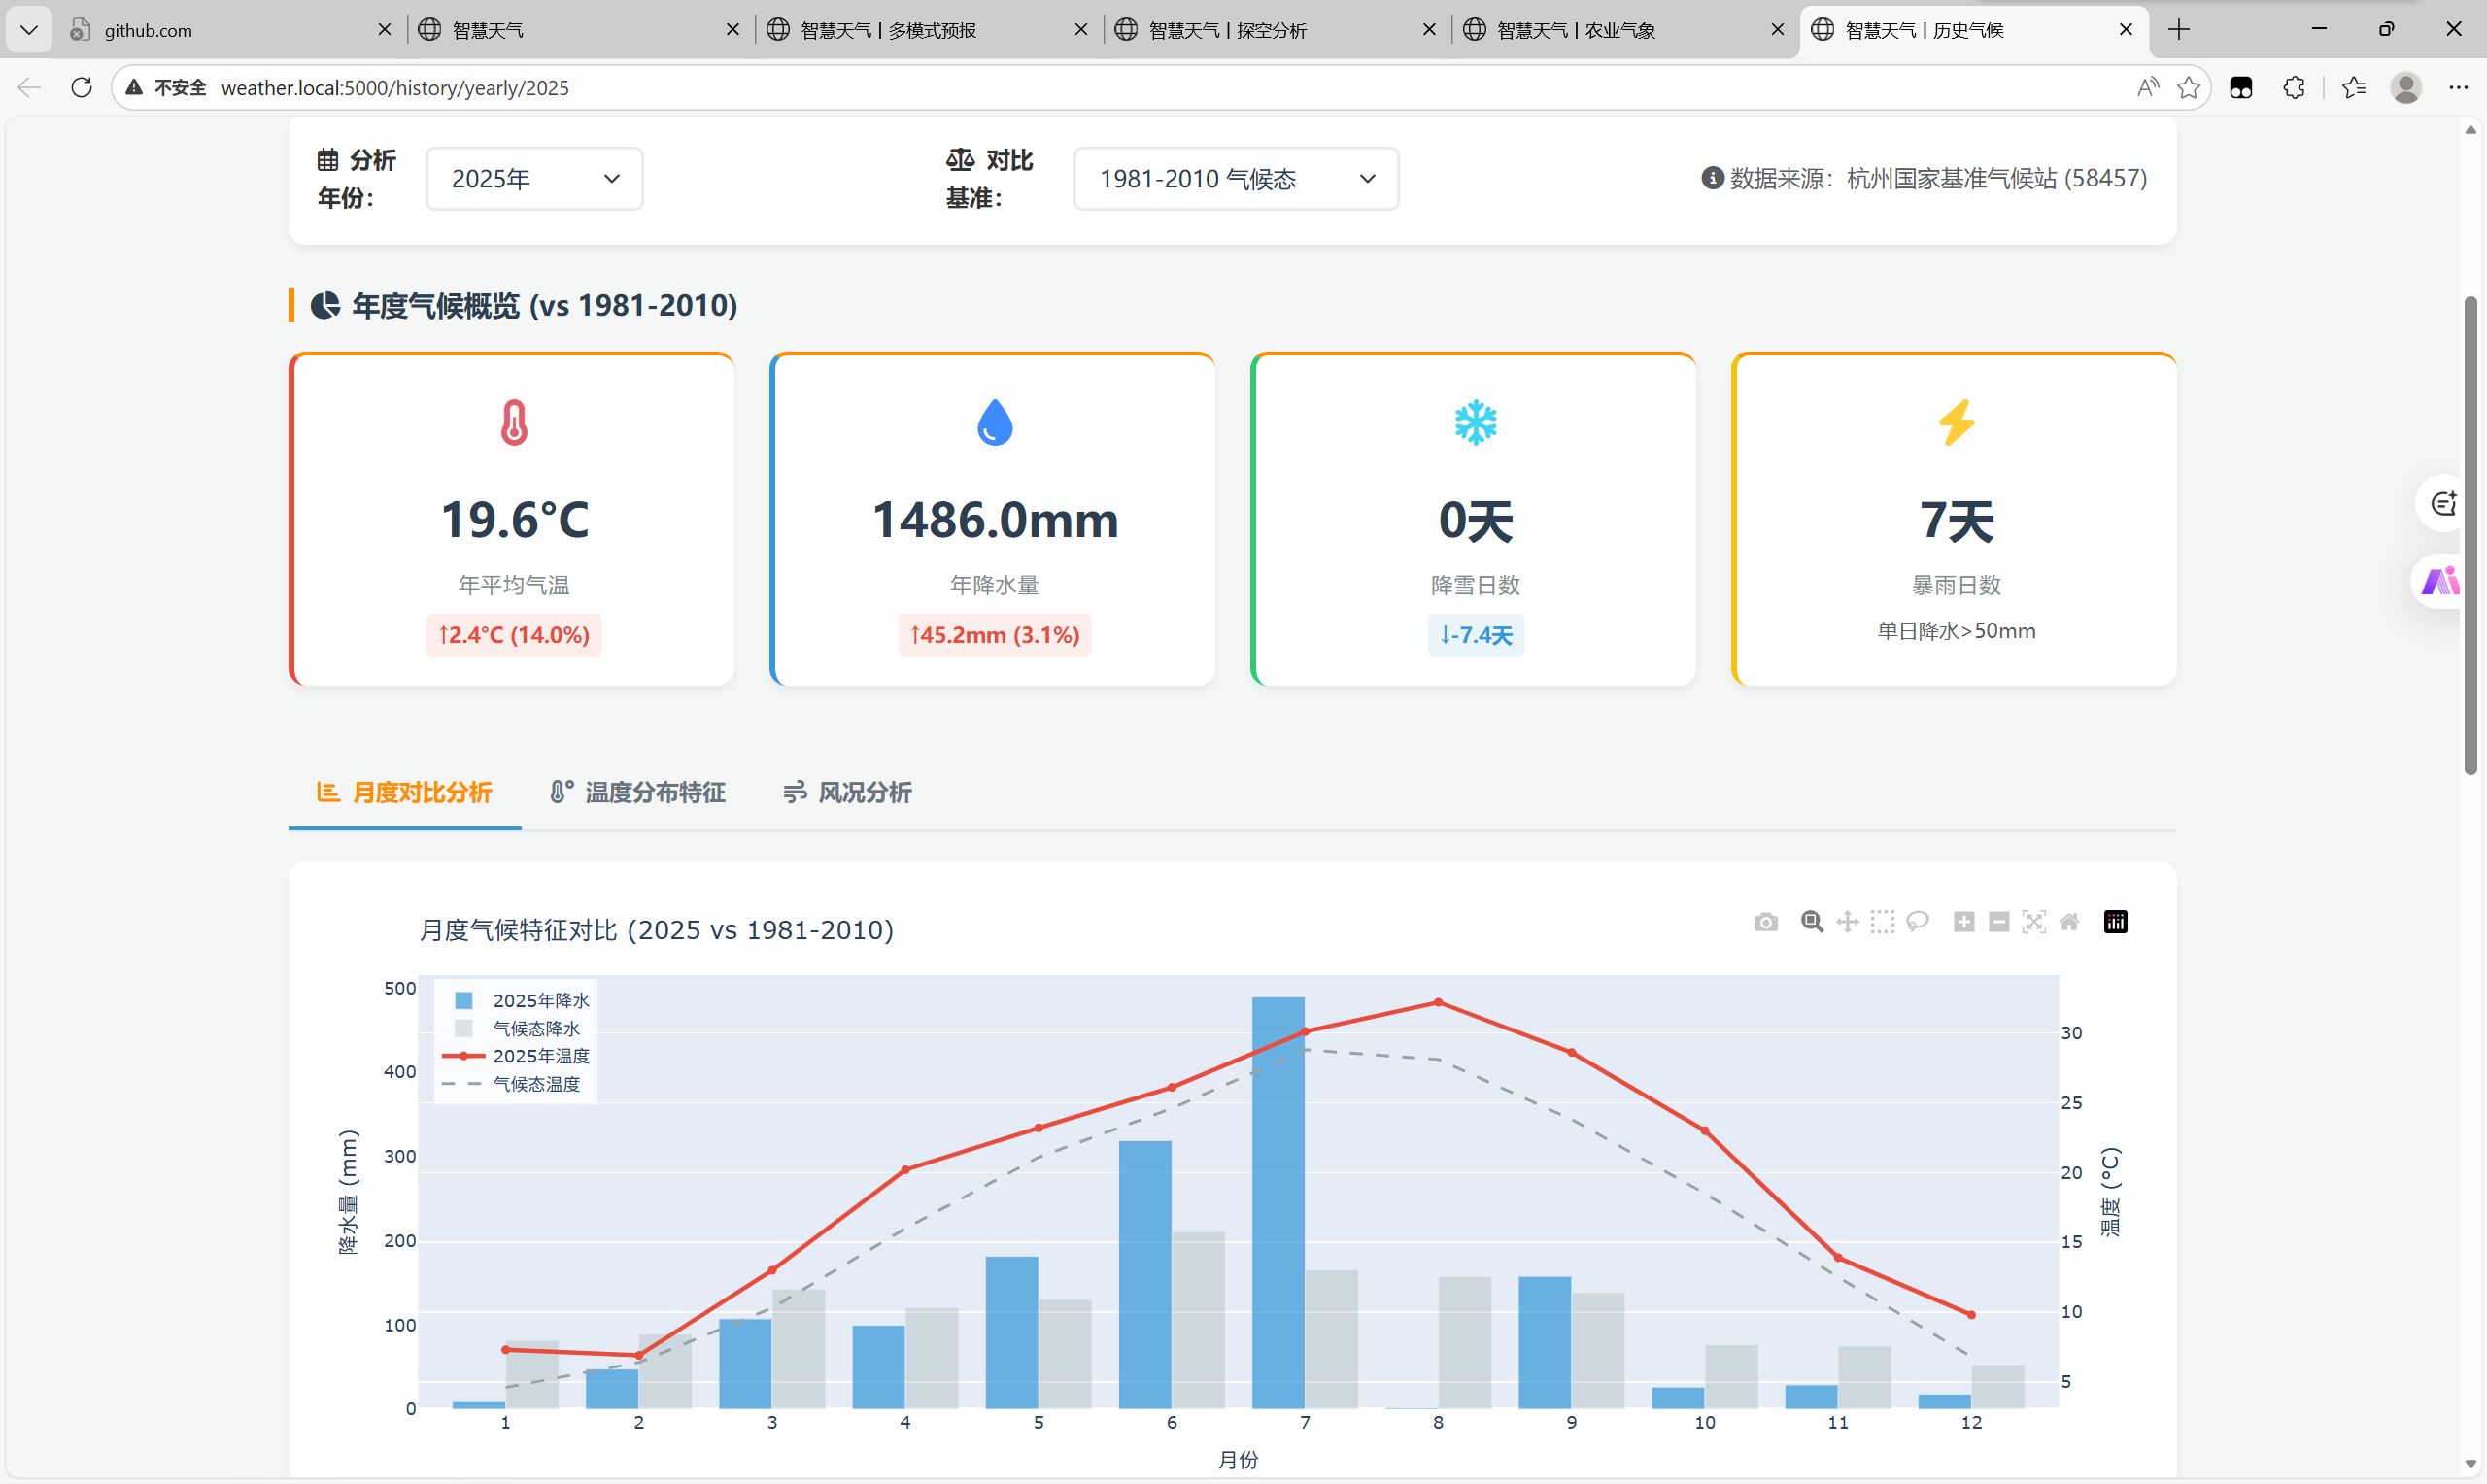
\includegraphics[width=\textwidth]{history.png}
      {\tiny 年度页（极端事件榜单）}
    \column{0.40\textwidth}
      \centering
      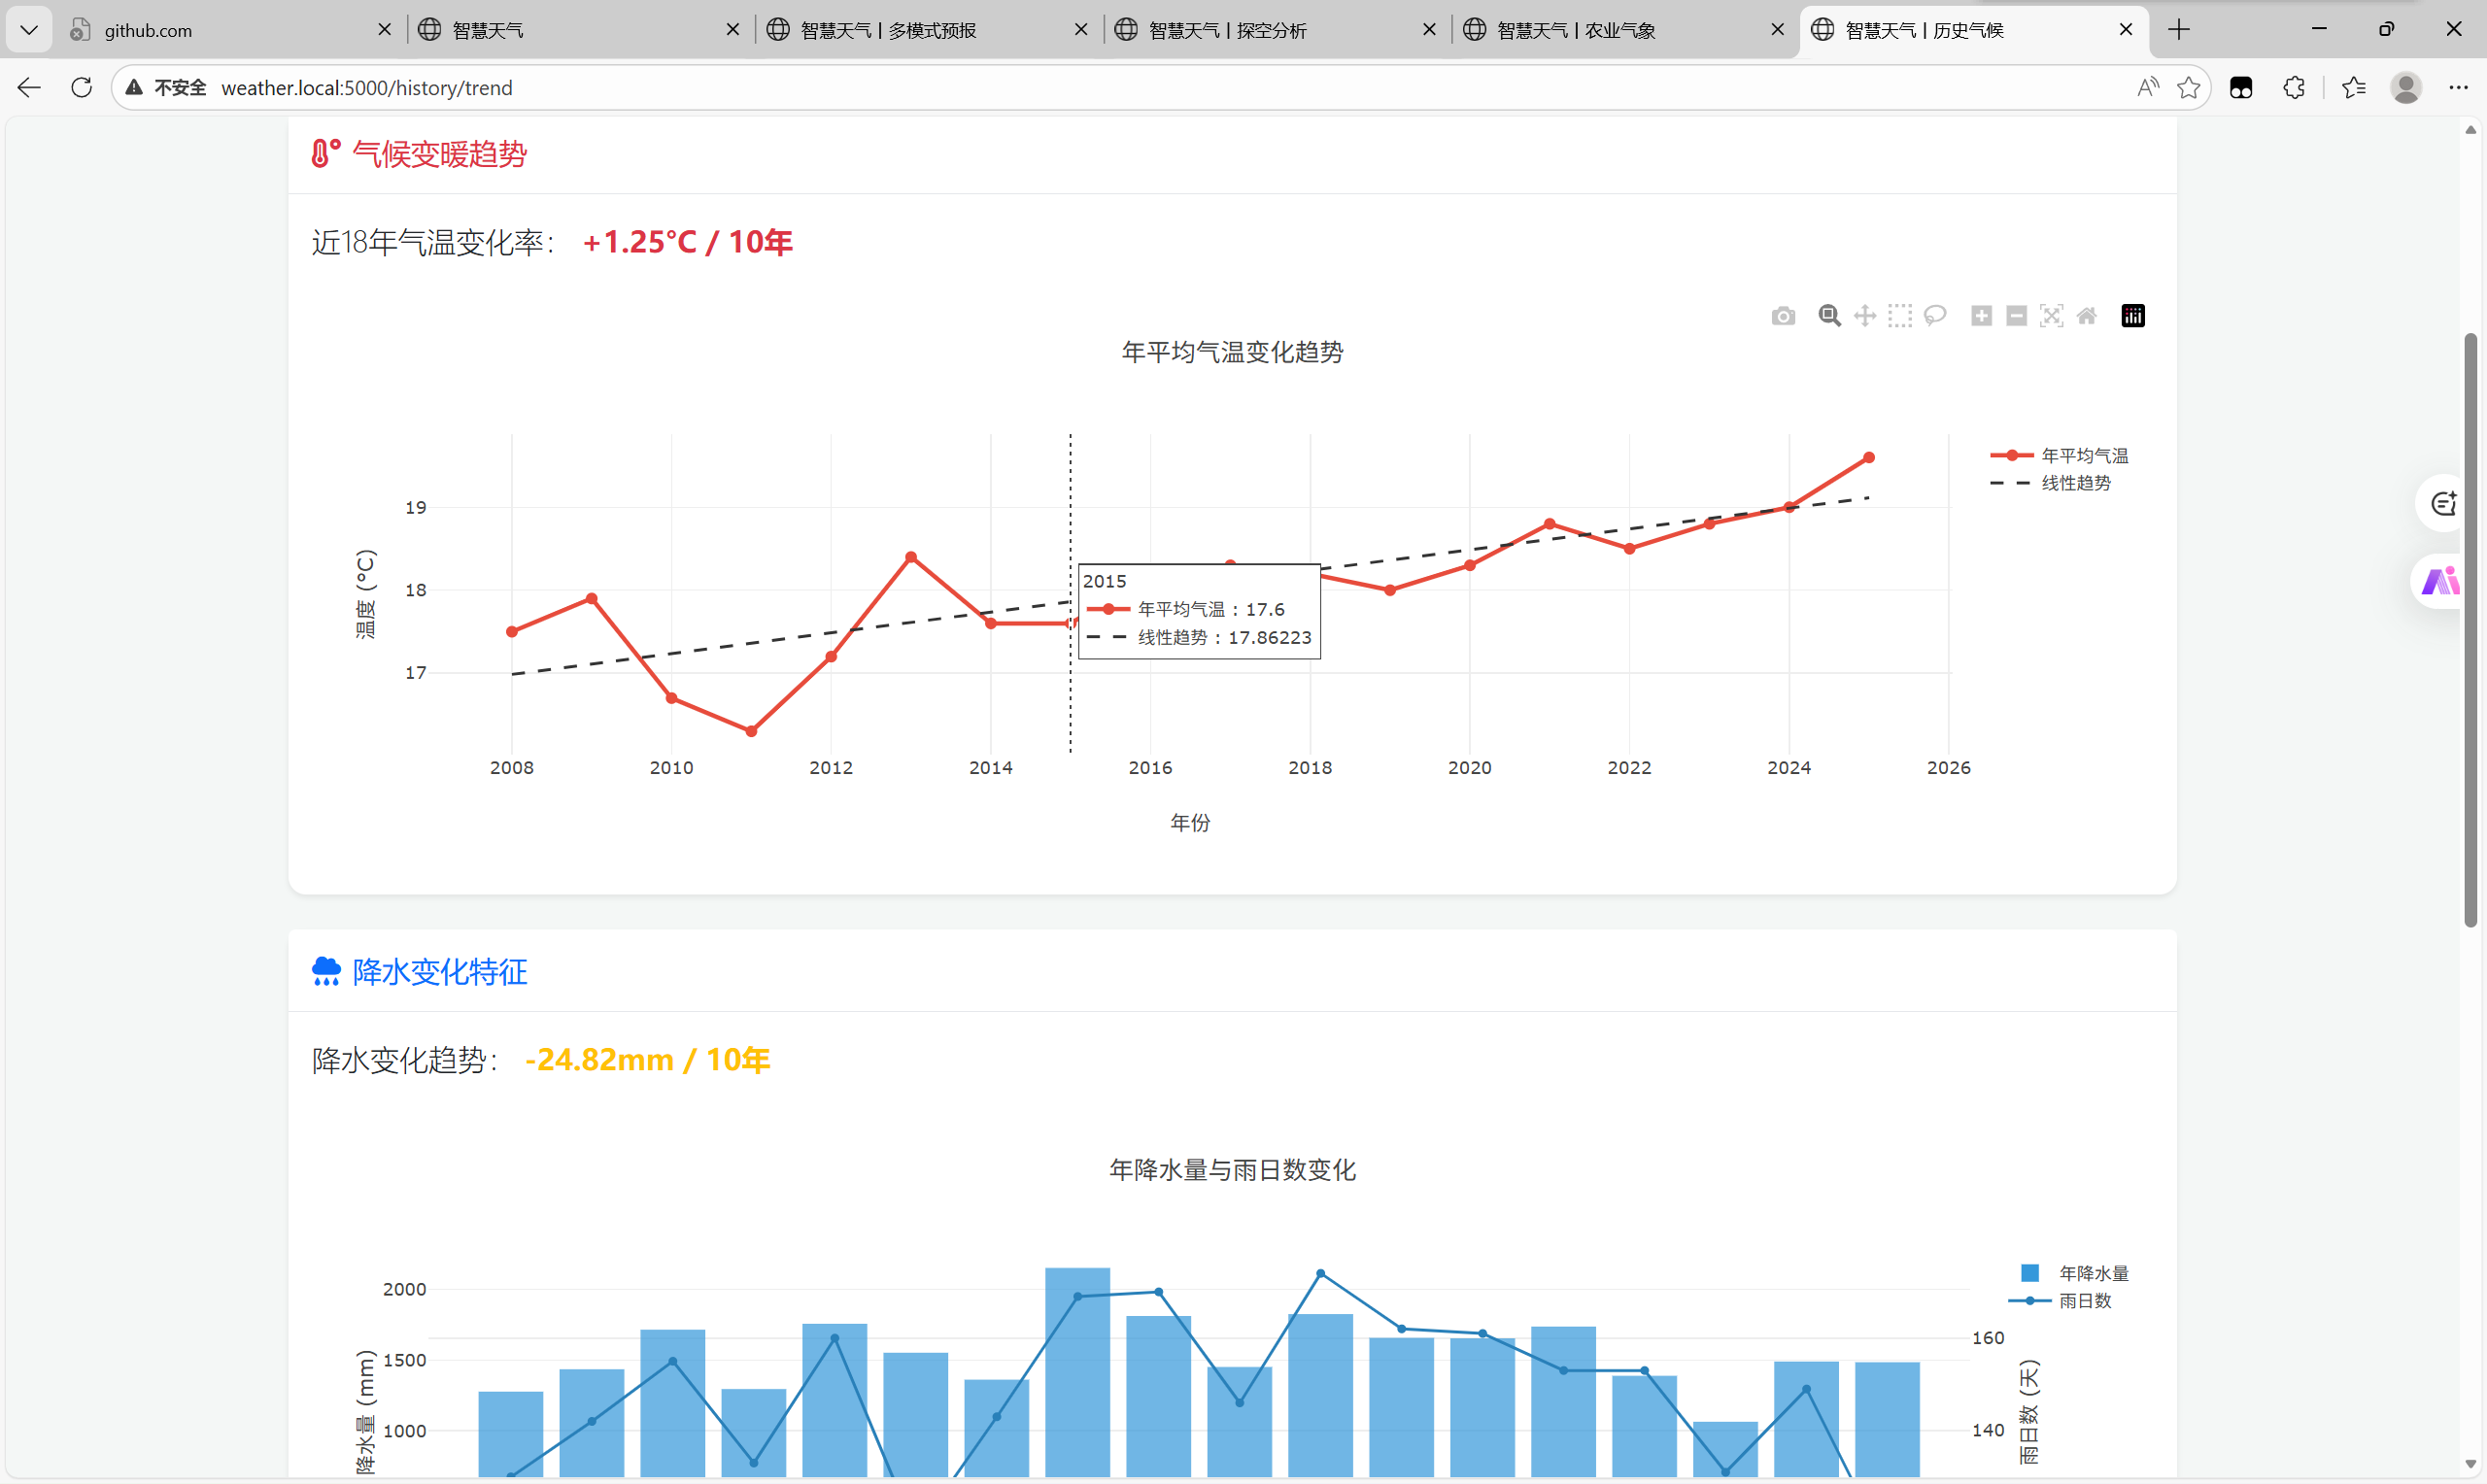
\includegraphics[width=\textwidth]{trend.png}
      {\tiny 长期趋势分析页}
  \end{columns}
  \vspace{2mm}
  \begin{itemize}
    \item 默认"原始极值"模式：按绝对值排序，直观易懂
    \item 一键切换"EW 指数"模式：按历史异常程度排序
    \item 四季分组 + 每季每要素限 3 条，避免单一季节占据全部榜单
  \end{itemize}
  \note{页面展示——默认极值榜，右上角可切换到EW指数模式。一次持续5天的高温过程在榜单中只出现最有代表性的那天。}
\end{frame}

% ═══════════════════════════════════════════
% 模块四：ML 误差校正（Slides 17-20）
% ═══════════════════════════════════════════
\section{机器学习误差校正模块}

\begin{frame}{ML 误差校正：修正 ECMWF 的系统性偏差}
  \begin{columns}[T]
    \column{0.52\textwidth}
      \begin{itemize}
        \item \textbf{问题}：ECMWF 全球模式在杭州单站\\{\small 存在系统性偏差（中远期偏暖、偏湿）}
        \item \textbf{不等于"不准"}：模式本身很好\\{\small 但落到具体站点需要后处理订正}
        \item \textbf{思路}：用历史预报 + 对应时次真实观测\\{\small $\rightarrow$ 训练模型学习偏差模式}
        \item \textbf{误差校正} = 让预报更接近\\{\small 这个站点的实际情况}
      \end{itemize}
    \column{0.43\textwidth}
      \centering
      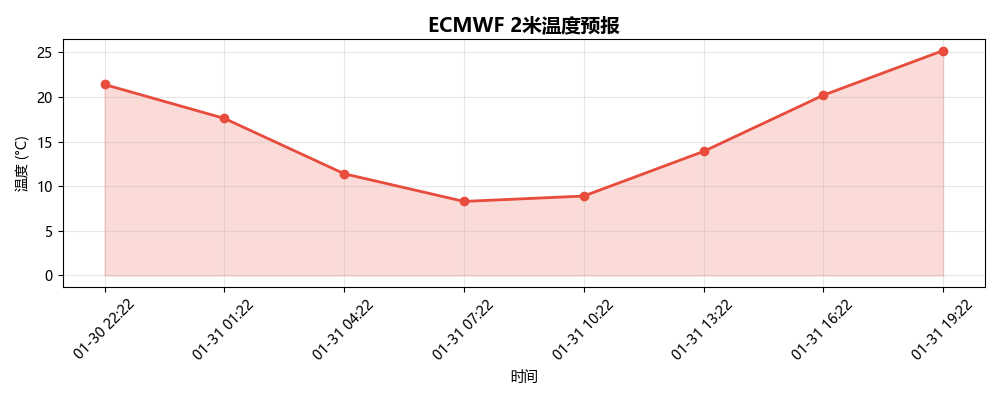
\includegraphics[width=\textwidth]{ecmwf_temp.png}
      {\tiny ECMWF 原始温度预报示意}
  \end{columns}
  \note{先讲清楚"校正"不是"推翻"——ECMWF是全球顶级模式，但任何全球模式落到一个城市站点都会有偏差。我要做的是训练模型学习"当ECMWF报25°C时实际杭州站大概23°C"。}
\end{frame}

\begin{frame}{训练流程：比模型选择更重要的是口径统一}
  \begin{columns}[T]
    \column{0.38\textwidth}
      \centering
      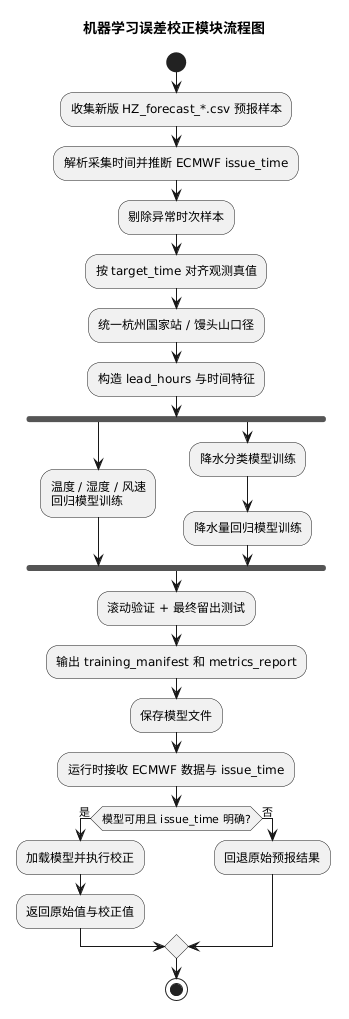
\includegraphics[width=\textwidth]{ml_correction_flow.png}
    \column{0.57\textwidth}
      \begin{itemize}
        \item \textbf{数据基础}：97 条新版 ECMWF 预报文件\\{\small（HZ\_forecast\_*.csv，3 条因时次不符剔除）}
        \item \textbf{训练切分}：按起报时间（issue\_time）切分\\{\small 严禁随机打散 $\rightarrow$ 杜绝信息泄漏}
        \item \textbf{V1 模型}：随机森林\\{\small 温度/湿度/风速：回归；降水：先分类后回归}
        \item \textbf{特征设计}：预报值 + 时间 + 时效 + 周期编码\\{\small V2 增强：季节/起报周期/3h-6h 变化率}
      \end{itemize}
  \end{columns}
  \note{最重要不是模型复杂度而是数据切分方式。按起报时间切分而不是随机打散——后者会让未来样本泄漏到训练集中导致评估虚高。97个文件中3个因采集时间不符合ECMWF起报窗口被剔除。}
\end{frame}

\begin{frame}{误差校正效果：三个连续变量明显改善}
  \centering
  \vspace{2mm}
  {\Large\textbf{连续变量 MAE 对比}}
  \vspace{4mm}
  \begin{tabular}{lccc}
    \toprule
    \textbf{气象要素} & \textbf{原始 ECMWF} & \textbf{校正后} & \textbf{改进幅度} \\
    \midrule
    温度 & 2.355°C & 1.832°C & \textcolor{highlight}{\textbf{$\downarrow$ 22.2\%}} \\
    湿度 & 9.851\% & 9.085\% & $\downarrow$ 7.8\% \\
    风速 & 4.413 m/s & 2.613 m/s & \textcolor{highlight}{\textbf{$\downarrow$ 40.8\%}} \\
    \bottomrule
  \end{tabular}
  \vspace{4mm}
  \begin{itemize}
    \item 短时效（1--3 天）改善更明显
    \item \textbf{降水}：分类指标基本持平，但\textbf{量级误差明显降低}\\{\small （策略偏保守——减少"报了雨但实际没下"的误报）}
  \end{itemize}
  \note{核心数据页。温度降0.5°C，风速改善最大因为原始ECMWF在杭州站的风速偏差本身就大。降水分类没全面提升但量级更准——对农业灌溉来说量级准比"下不下"的准确率更重要。}
\end{frame}

\begin{frame}{V1 vs V2：小样本下的真实对比}
  \centering
  \vspace{2mm}
  {\Large\textbf{三版本对比（严格时间隔离测试集）}}
  \vspace{3mm}
  \begin{tabular}{lcccc}
    \toprule
    \textbf{指标} & \textbf{原始 ECMWF} & \textbf{V1 (RF)} & \textbf{V2 (CatBoost)} \\
    \midrule
    温度 MAE & 2.355 & \textcolor{highlight}{\textbf{1.832}} & 2.220 \\
    湿度 MAE & 9.851 & \textcolor{highlight}{\textbf{9.085}} & 10.076 \\
    风速 MAE & 4.413 & \textcolor{highlight}{\textbf{2.613}} & 3.061 \\
    降水 Acc & 0.754 & 0.743 & 0.658 \\
    \bottomrule
  \end{tabular}
  \vspace{4mm}
  \begin{itemize}
    \item V2 未优于 V1 —— \textbf{合理且诚实的结果}
    \item 原因：约 2 个月样本，bagging（RF）天然比\\boosting（CatBoost）在小样本下更稳定
    \item \textbf{核心结论：口径统一比换复杂模型更重要}
  \end{itemize}
  \note{V2用CatBoost反而比V1差——不是失败。小样本下RF天然比boosting更稳定。核心结论是口径统一比模型复杂度对结果可信度的提升更大。如果以后积累一整年数据再重新评估boosting才公平。}
\end{frame}

% ═══════════════════════════════════════════
% 模块五：农业气象服务（Slides 21-23）
% ═══════════════════════════════════════════
\section{农业气象服务模块}

\begin{frame}{农业气象：从天气数据到田间决策}
  \begin{columns}[T]
    \column{0.42\textwidth}
      \centering
      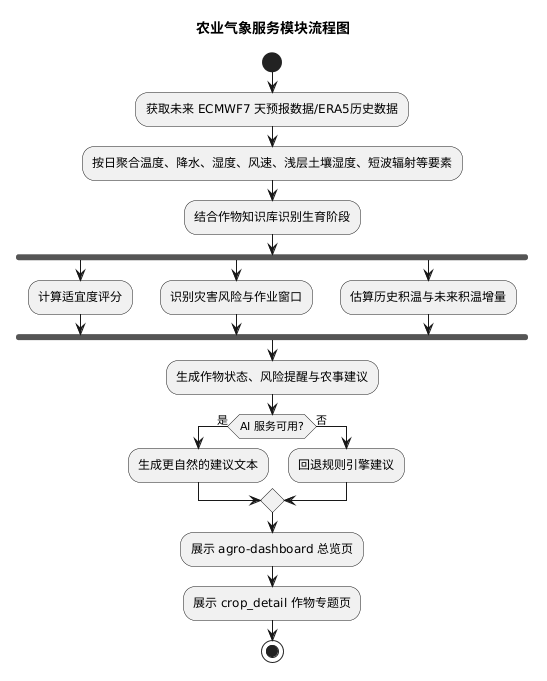
\includegraphics[width=\textwidth]{agro_service_flow.png}
    \column{0.53\textwidth}
      \begin{itemize}
        \item \textbf{5 种浙江代表作物}：\\{\small 单季晚稻 / 西湖龙井 / 杨梅 / 柑橘 / 小白菜}
        \item \textbf{作物知识库}：生育阶段 + 温度阈值\\{\small + 积温参数 + 气象风险定义}
        \item \textbf{四核心输出}：\\作物状态 $\rightarrow$ 适宜度评分 $\rightarrow$ 风险预警 $\rightarrow$ AI 建议
        \item \textbf{积温}：历史 ERA5-Land + 未来 ECMWF\\{\small （双侧优势互补）}
      \end{itemize}
  \end{columns}
  \note{农业模块是"最后一公里"。每种作物有知识库——西湖龙井最怕倒春寒、杨梅成熟期最怕暴雨大风。积温历史用再分析（长期稳定）、未来用ECMWF（时效性强），两边发挥各自优势。}
\end{frame}

\begin{frame}{农业仪表盘：一眼掌握全局}
  \begin{columns}[T]
    \column{0.58\textwidth}
      \centering
      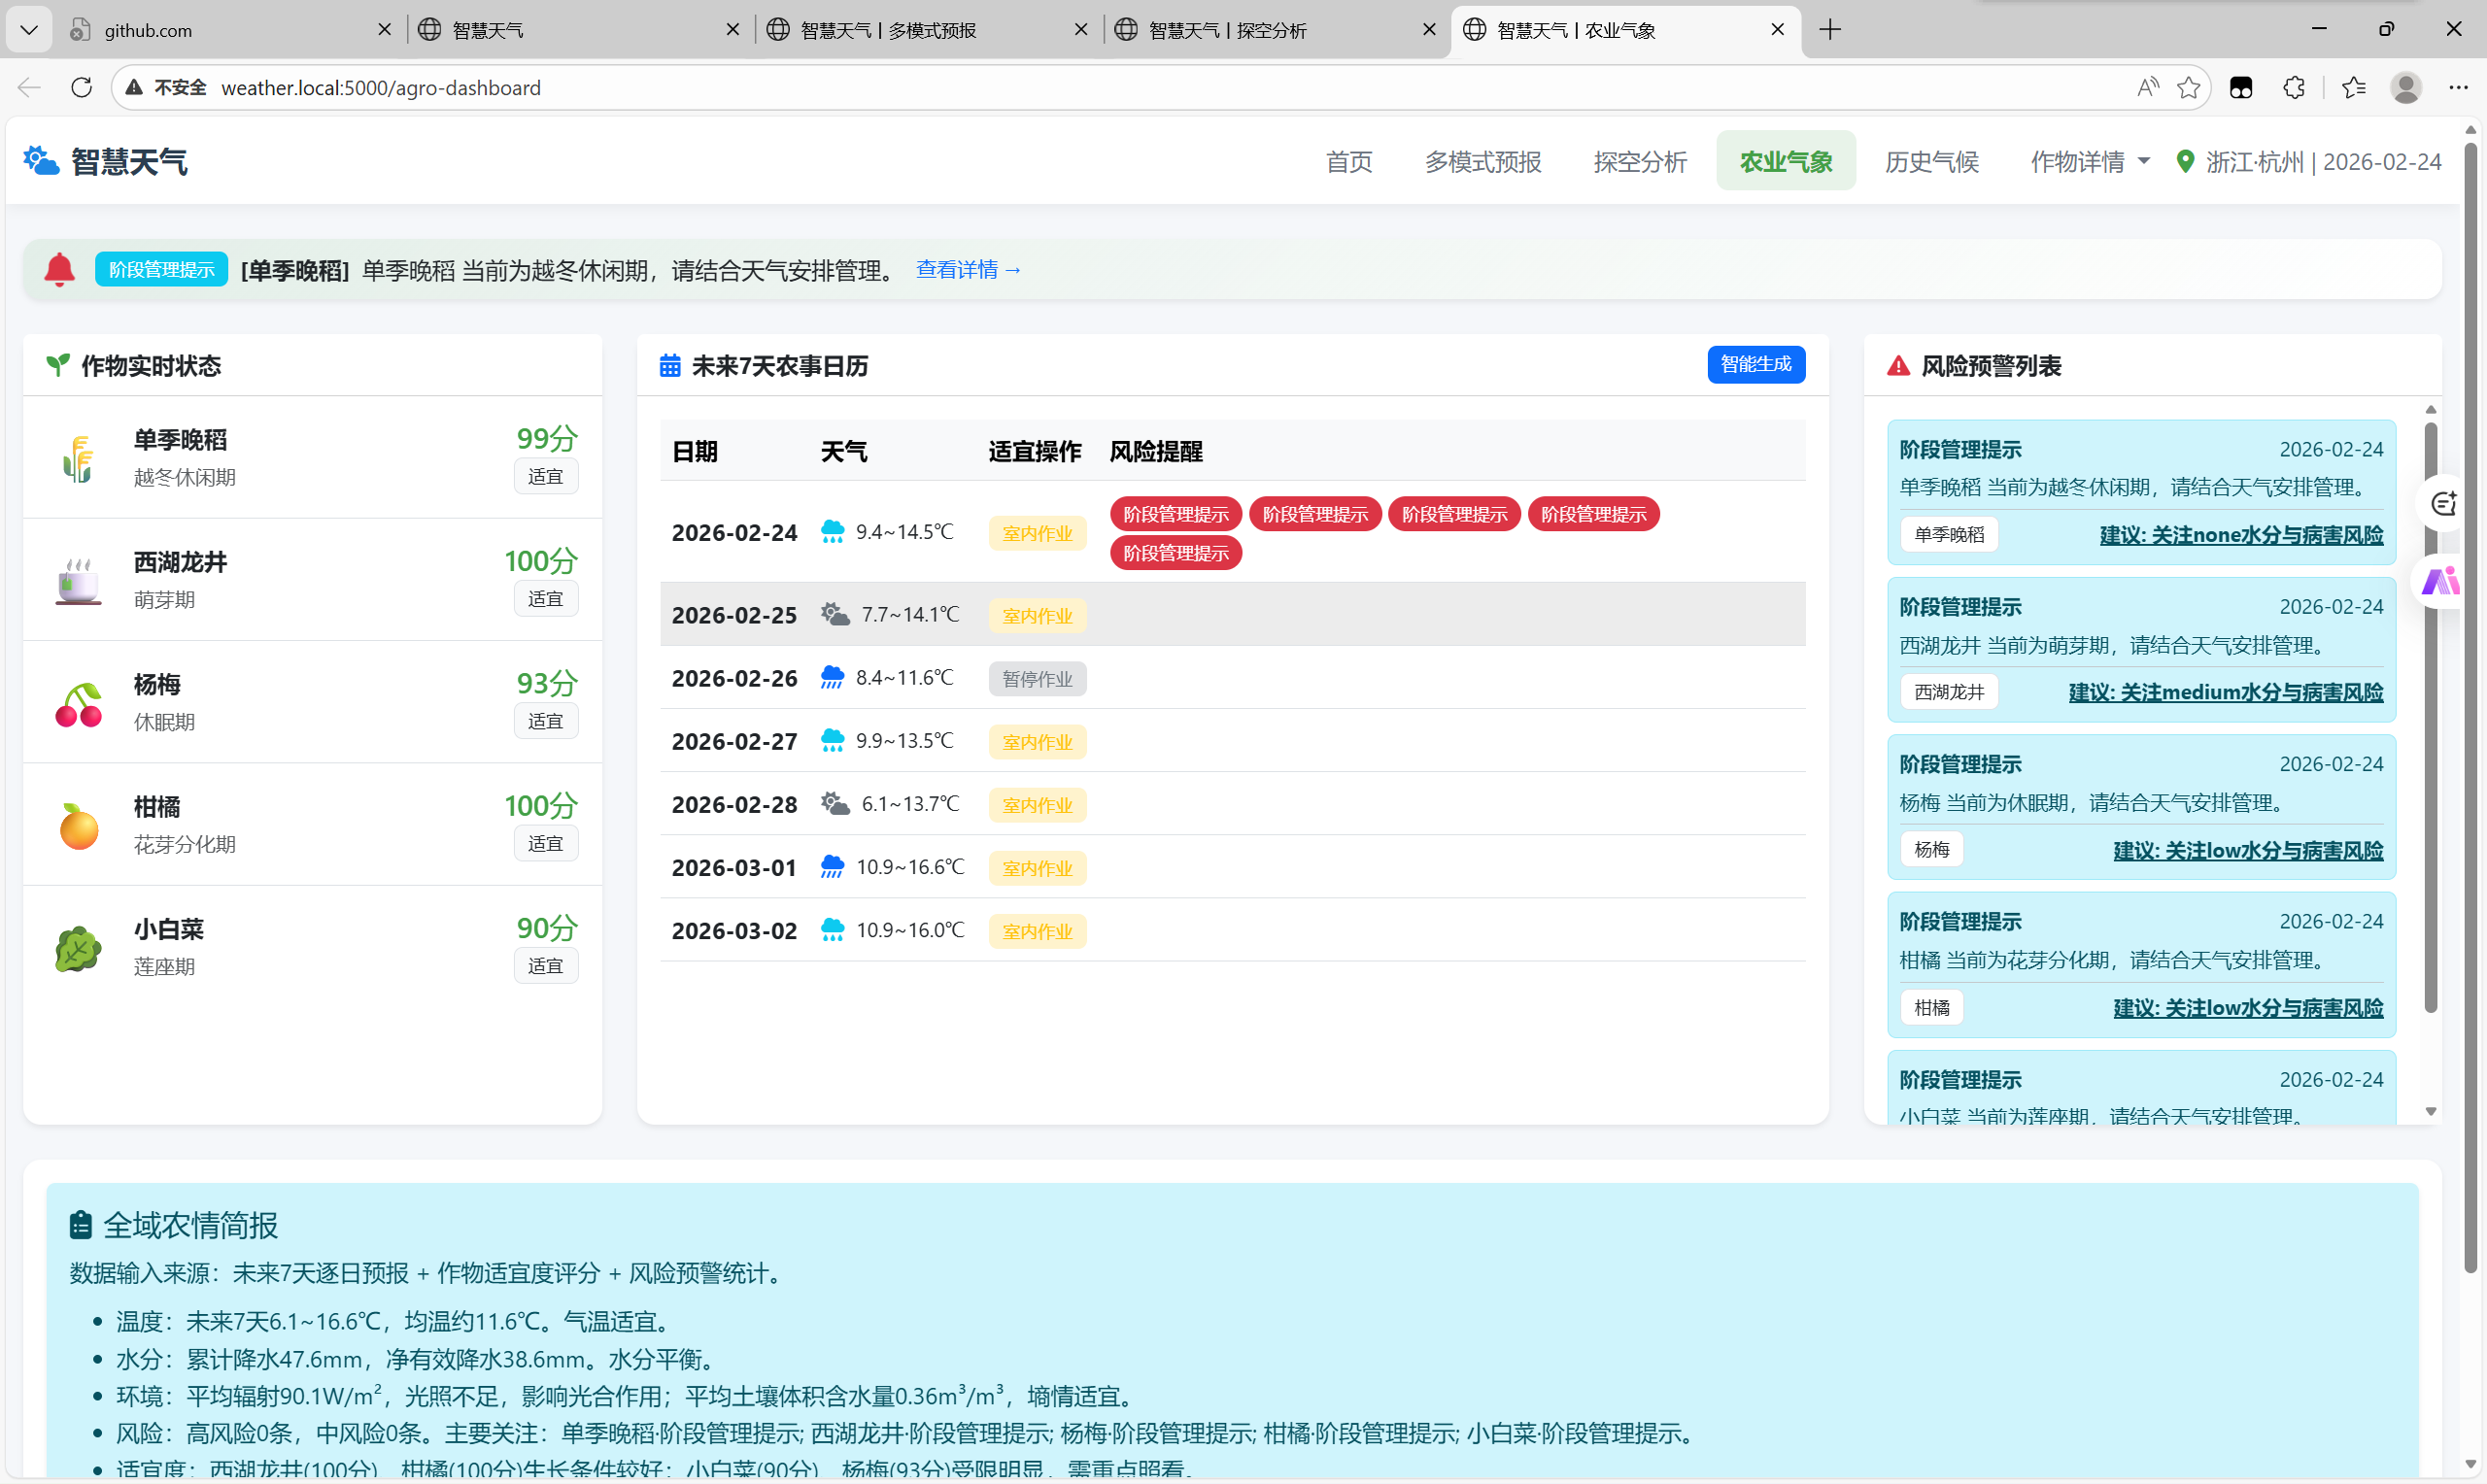
\includegraphics[width=\textwidth]{agro-dashboard.png}
      {\tiny 农业气象总览页}
    \column{0.38\textwidth}
      \centering
      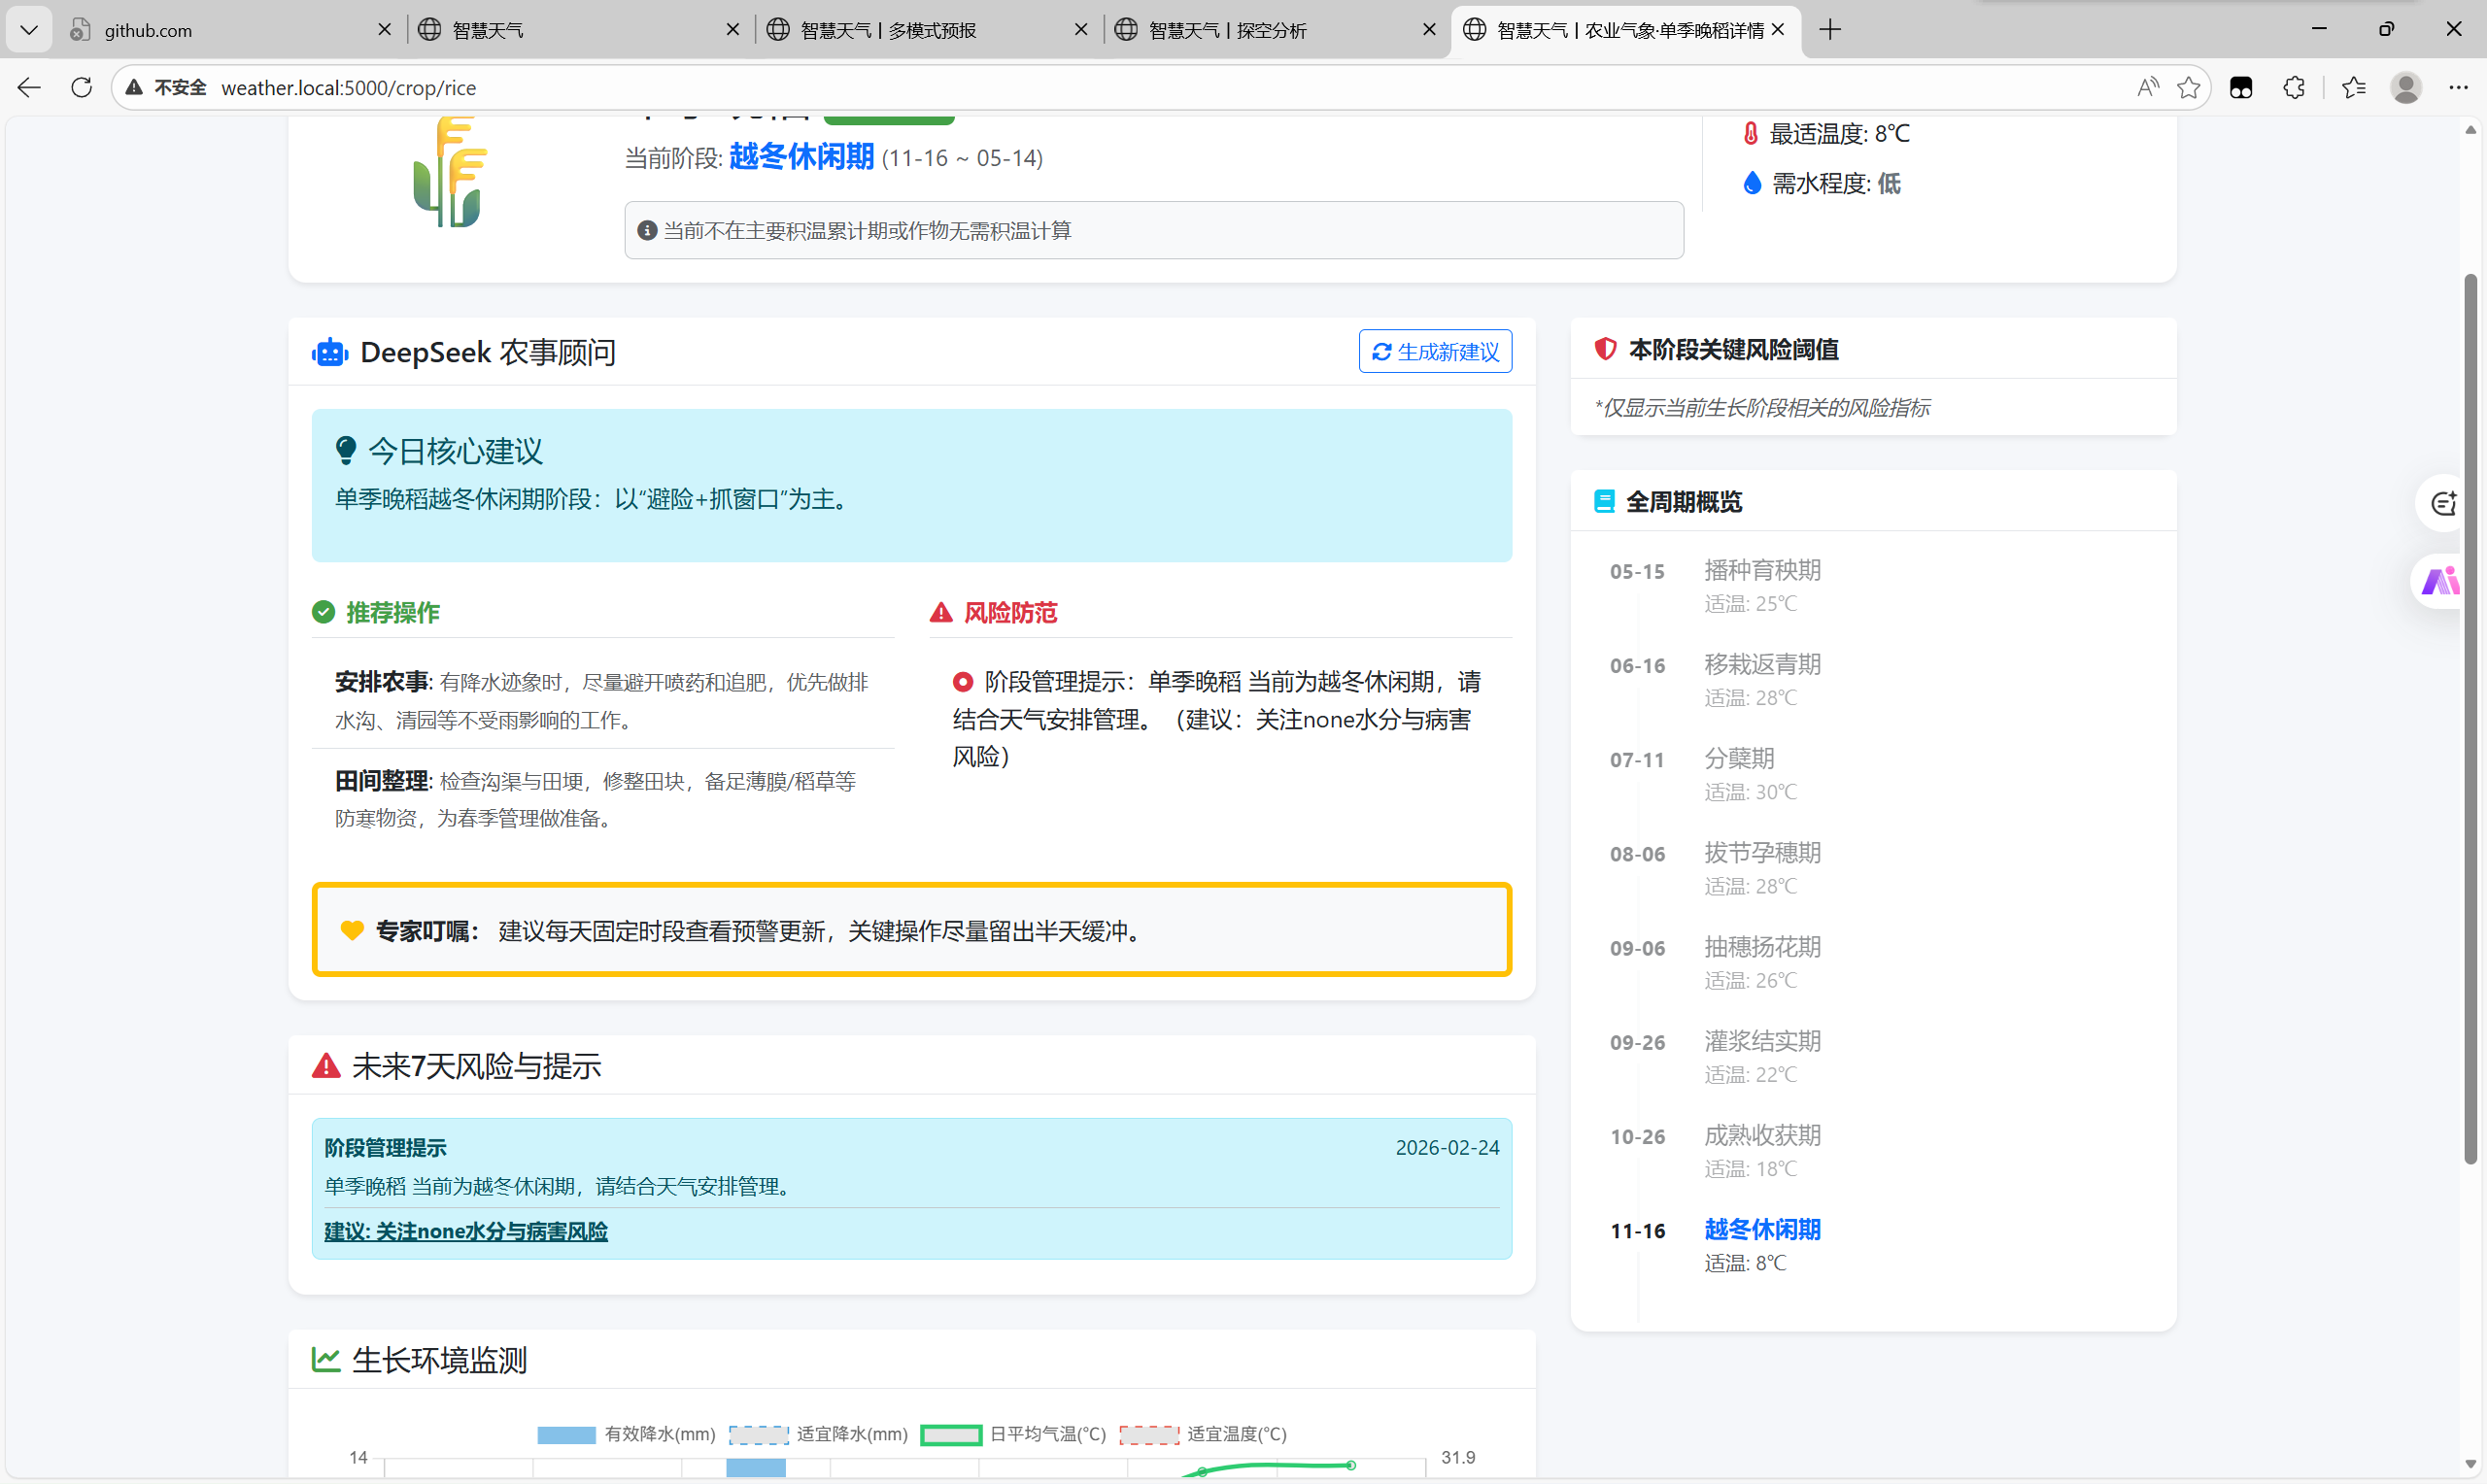
\includegraphics[width=\textwidth]{rice.png}
      {\tiny 水稻专题页}
  \end{columns}
  \vspace{2mm}
  \begin{itemize}
    \item 总览页：风险滚动条 + 作物状态 + 7 天农事日历 + 全局研判
    \item AI 建议 + 规则引擎双路径（DeepSeek API 不可用时自动切换）
    \item 专题页：积温进度条 + 环境曲线 + 逐日风险预警
  \end{itemize}
  \note{总览页给管理者快速看——哪些作物有风险、处于什么阶段。水稻专题页看积温进度和未来天气。AI建议不是唯一依赖，接口挂了自动切规则引擎。}
\end{frame}

\begin{frame}{积温计算 + 作物风险案例}
  \begin{columns}[T]
    \column{0.48\textwidth}
      \centering
      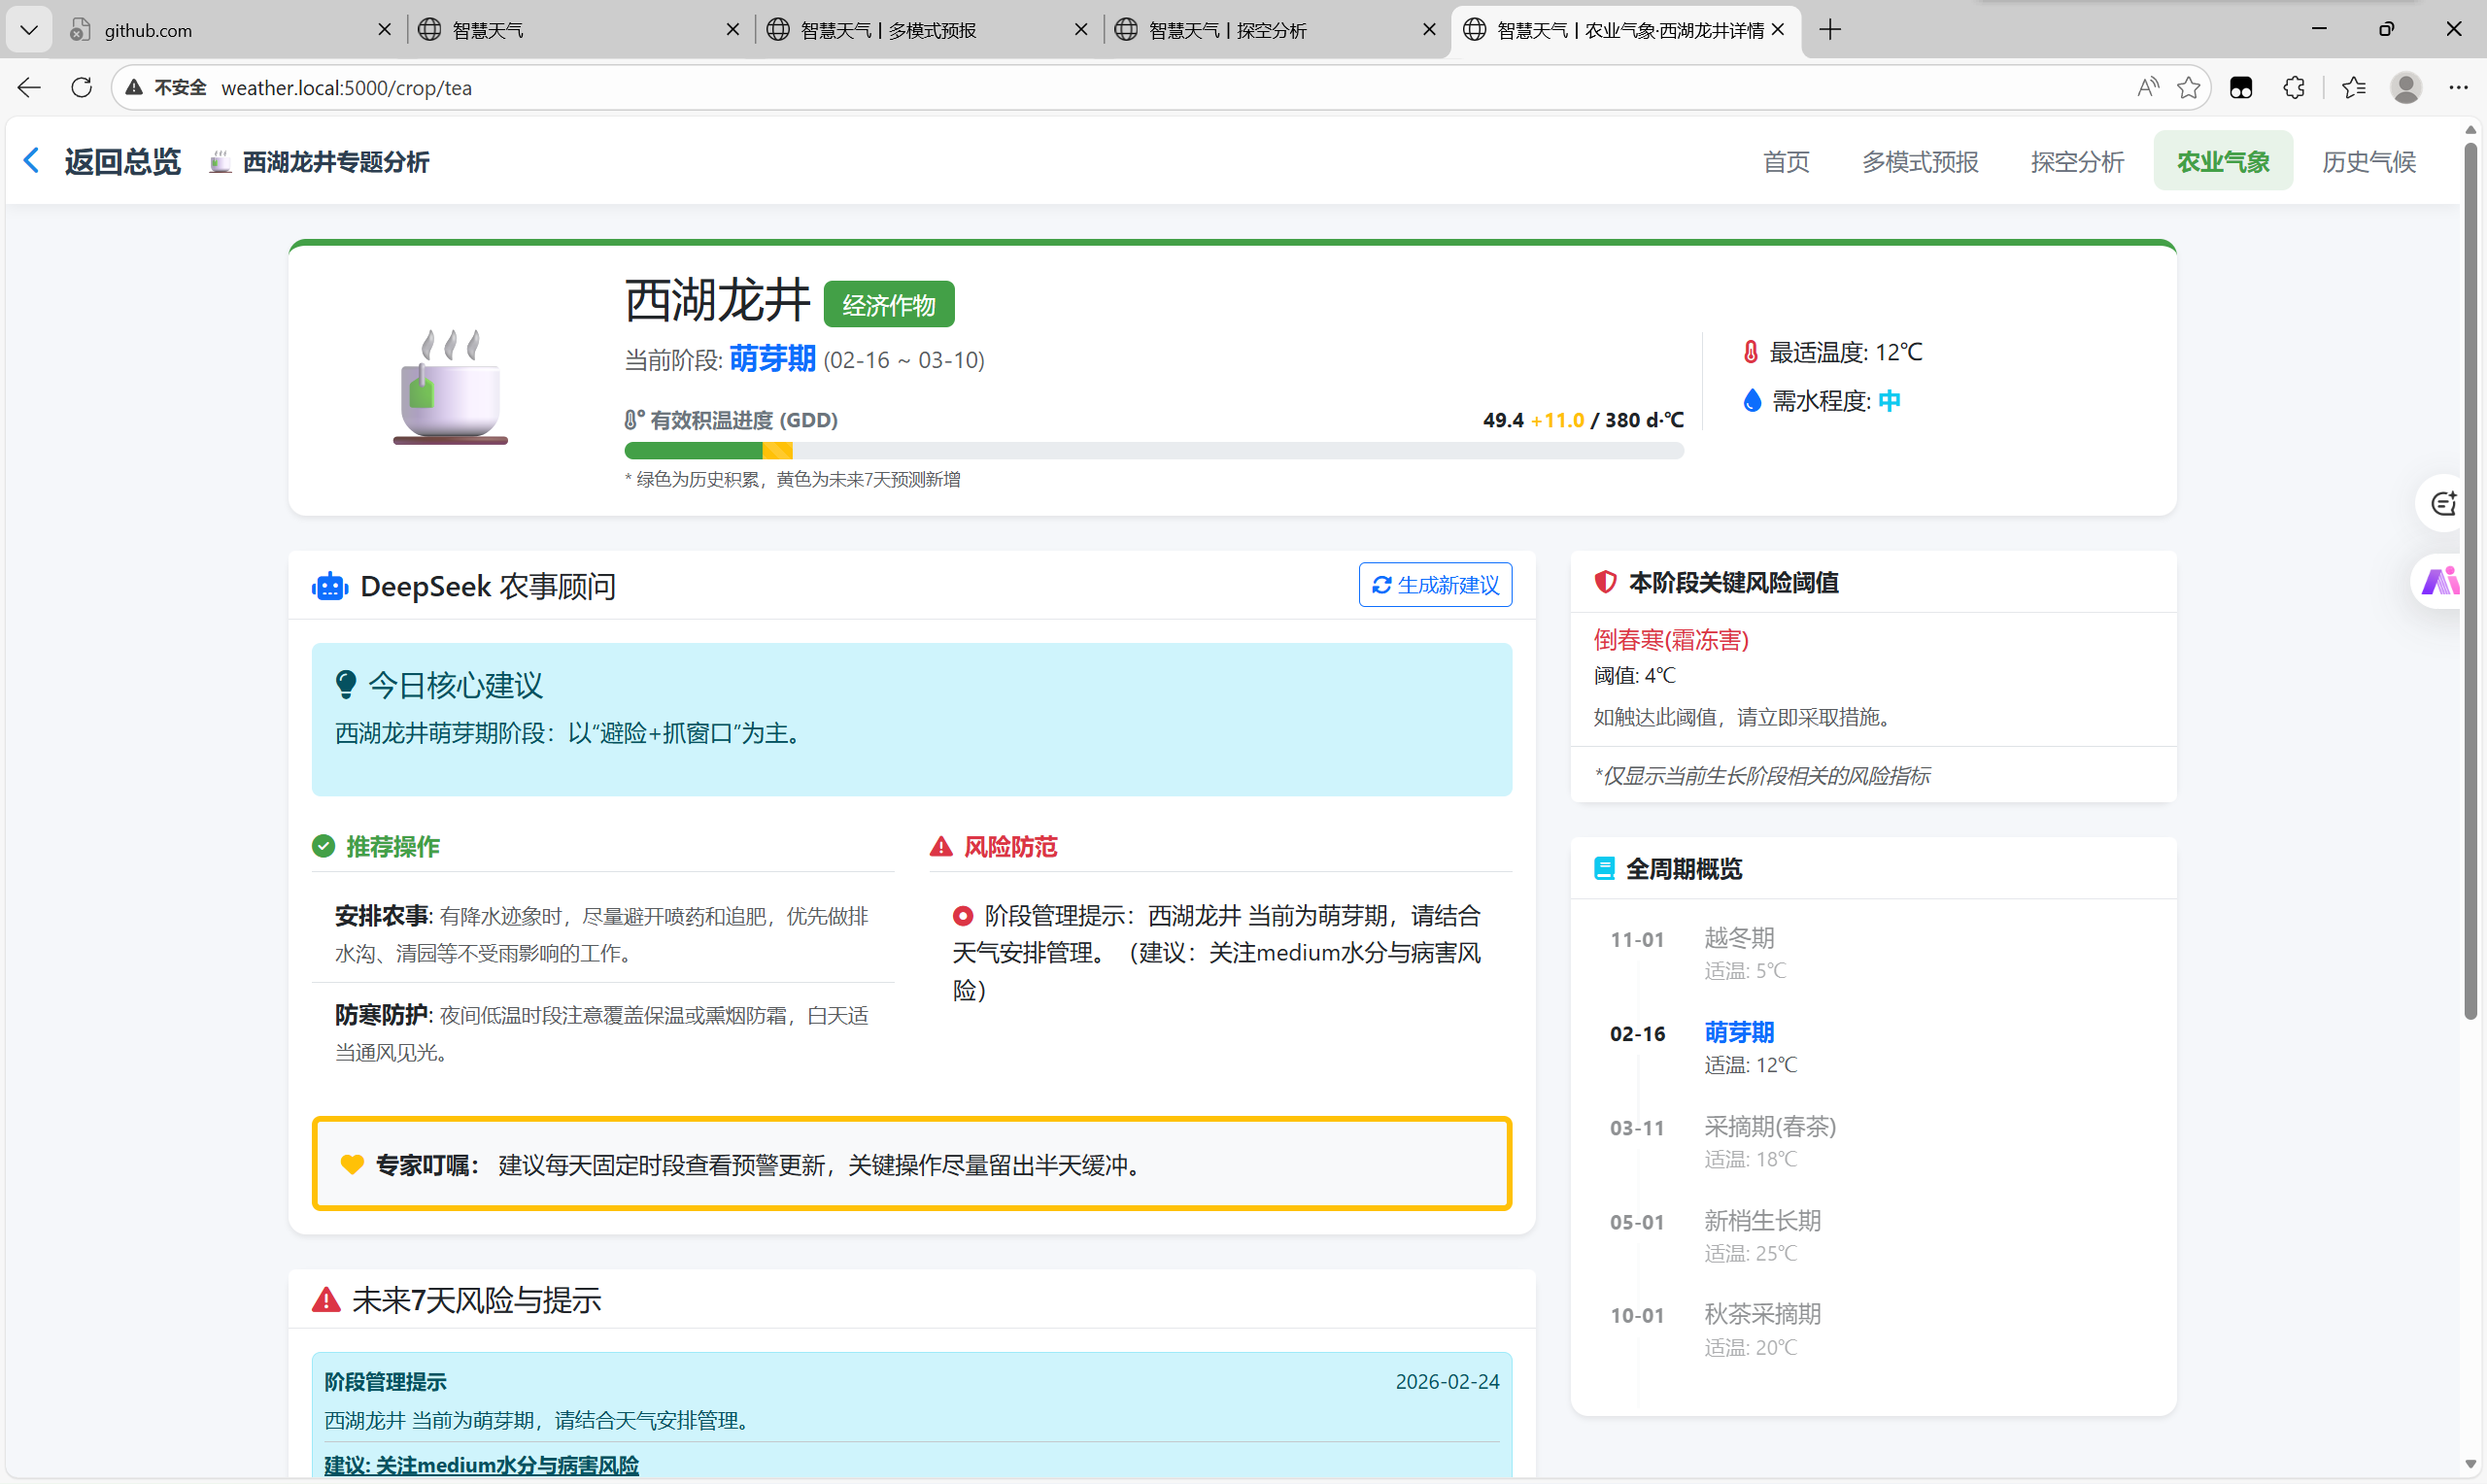
\includegraphics[width=\textwidth]{tea.png}
      {\tiny 西湖龙井专题页}
    \column{0.48\textwidth}
      \centering
      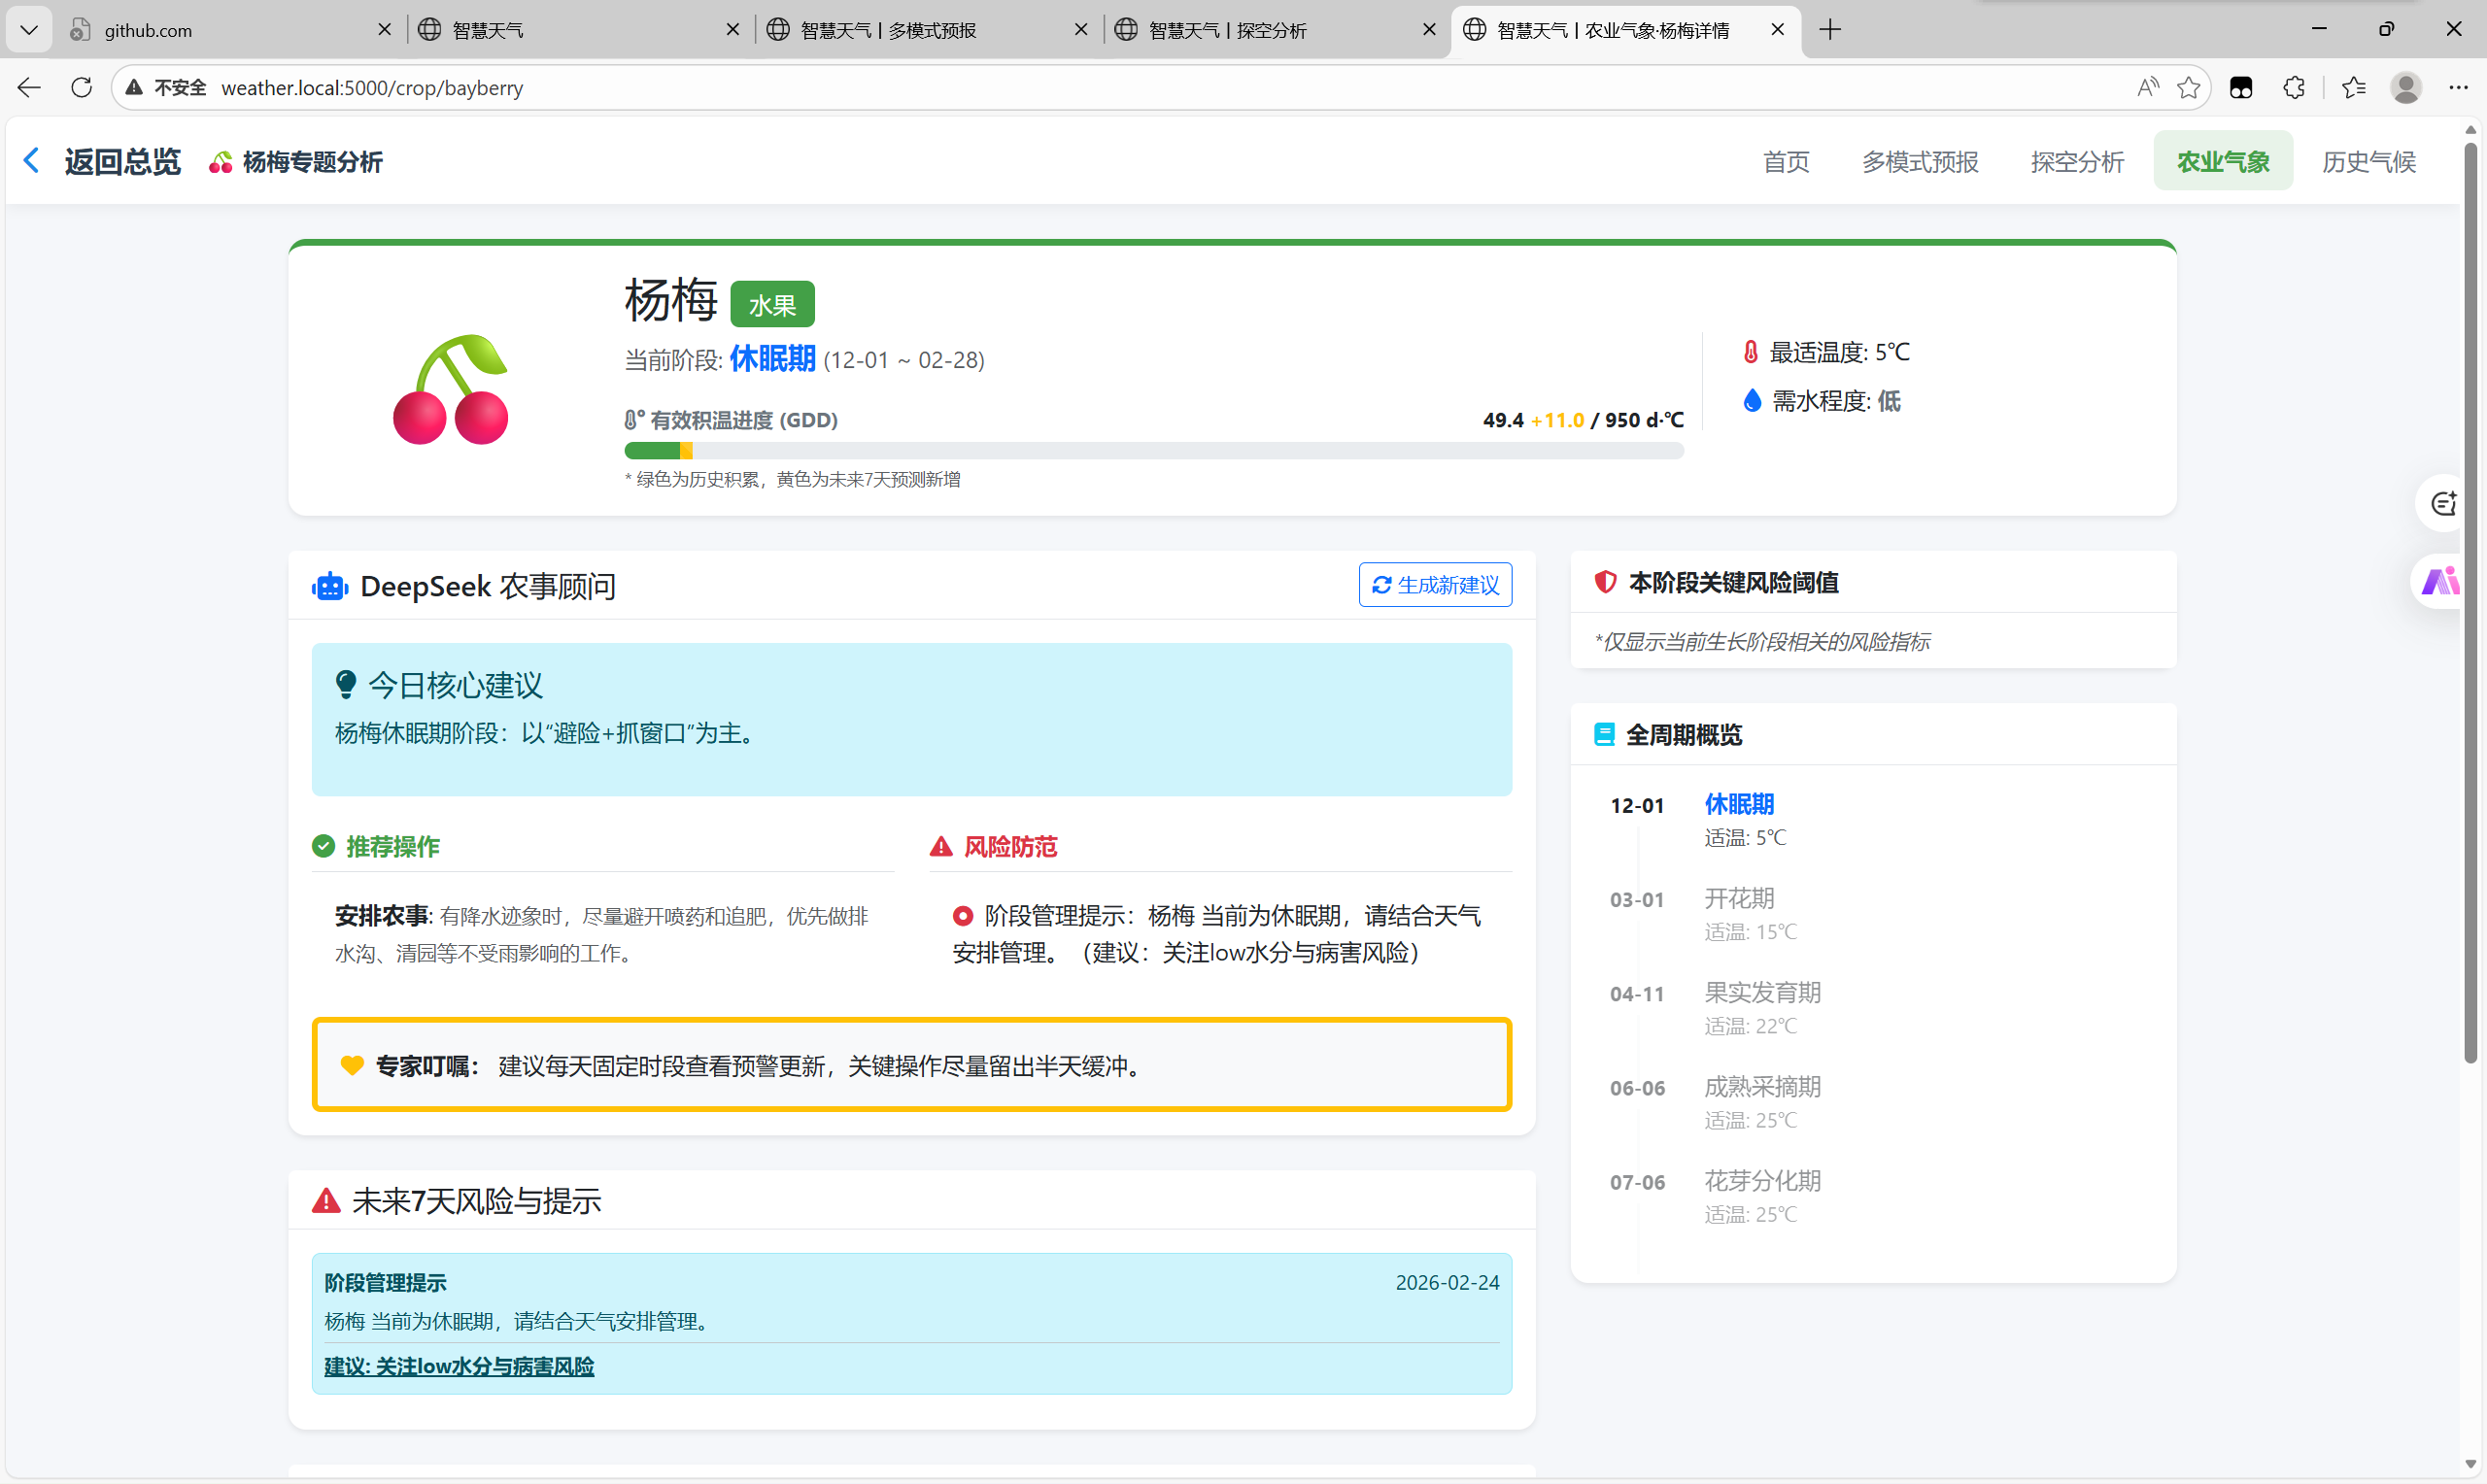
\includegraphics[width=\textwidth]{bayberry.png}
      {\tiny 杨梅专题页}
  \end{columns}
  \vspace{2mm}
  \begin{itemize}
    \item \textbf{积温方案}：ERA5-Land（起算日$\rightarrow$昨日）+ ECMWF（今日$\rightarrow$7天后）
    \item 西湖龙井：倒春寒（3--4 月）、高温灼伤（7--8 月）
    \item 杨梅：成熟期暴雨大风 $\rightarrow$ 落果烂果
    \item 不只报风险，同时识别\textbf{适合作业的窗口}（趋利避害并重）
  \end{itemize}
  \note{积温为什么混用两个数据源——历史需要长期连续（再分析优势），未来需要时效性（ECMWF优势）。系统不只报风险也会识别适合喷药施肥的窗口期，趋利和避害并重。}
\end{frame}

% ═══════════════════════════════════════════
% 收尾：测试 + 总结 + 致谢（Slides 24-26）
% ═══════════════════════════════════════════
\section{总结与展望}

\begin{frame}{系统测试：不只是"页面能打开"}
  \begin{columns}[T]
    \column{0.55\textwidth}
      \begin{itemize}
        \item \textbf{功能流程}：5 大模块页面/接口正常，业务链路闭环
        \item \textbf{EW 事件筛选}：过程去重/季节分组/数量控制正确
        \item \textbf{探空异常处理}：北京时间$\rightarrow$UTC 换算正确，\\CAPE 负值 $\rightarrow$ N/A
        \item \textbf{时次推断稳定}：\\04:15 采集 $\rightarrow$ 前日 12Z\\16:15 采集 $\rightarrow$ 当日 00Z
        \item \textbf{ML 评估可追溯}：97 训练/3 剔除，\\training\_manifest.json + metrics\_report.json
      \end{itemize}
    \column{0.40\textwidth}
      \centering
      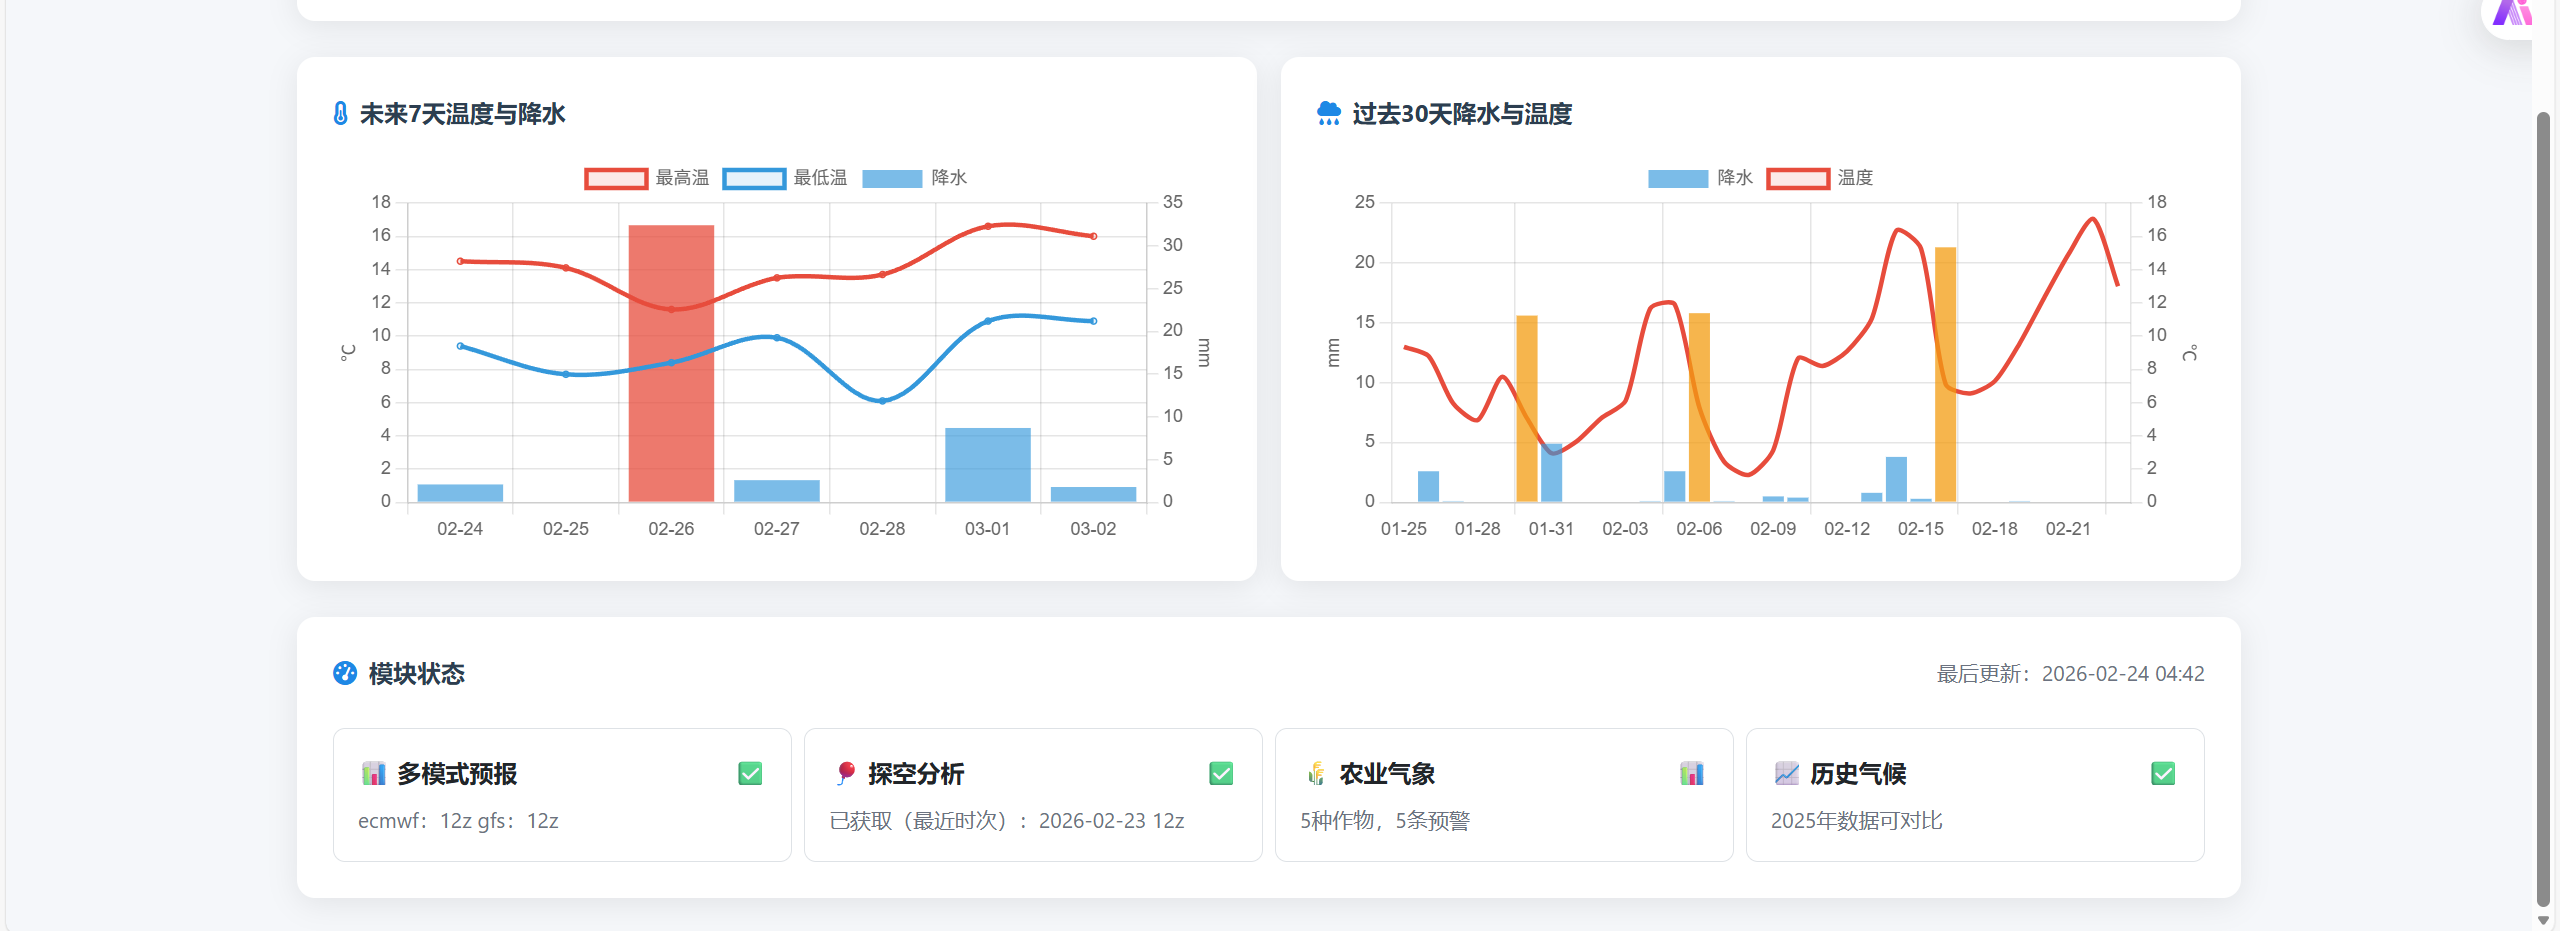
\includegraphics[width=\textwidth]{home2.png}
      {\tiny 首页智能提醒区（验证环境）}
  \end{columns}
  \note{这些验证可能不像模型数据表那么亮眼，但对运行系统最关键——时次推断错了ML校正口径就不一致；CAPE异常值没处理好就给用户误导数字。这些细节是系统可信度的基础。}
\end{frame}

\begin{frame}{总结：围绕真实场景的完整工程闭环}
  \begin{itemize}
    \item 完成了"预报展示 $\rightarrow$ 专业诊断 $\rightarrow$ 历史背景\\\hspace{6mm}$\rightarrow$ ML 后处理 $\rightarrow$ 行业应用"的完整平台
    \item \textbf{核心能力}：
      \begin{itemize}
        \item 多模式预报对比（ECMWF/GFS/ICON 三模式同轴）
        \item EW 指数代表事件识别（历史同日比较 + 过程去重）
        \item ML 误差校正（温度 $\downarrow$22.2\%、风速 $\downarrow$40.8\%）
        \item 农业气象行业闭环（5 种作物，积温/适宜度/风险/AI）
      \end{itemize}
    \item 不是追求单一算法创新，而是\textbf{组织可运行、可解释、可追溯的综合系统}
  \end{itemize}
  \note{最核心的Takeaway——这个系统不是靠单一算法体现价值，而是把多源数据、分析方法、可视化和误差校正整合成工程闭环。从用户打开首页到查多模式预报到ML校正到农事建议，整个链条是打通的。}
\end{frame}

\begin{frame}{不足、展望与致谢}
  \begin{columns}[T]
    \column{0.48\textwidth}
      \textbf{\textcolor{primary}{当前不足}}
      \begin{itemize}
        \item 数据源依赖外部\\{\small（Open-Meteo/怀俄明大学）}
        \item 训练样本仅约 2 个月\\{\small （持续采集后可重训）}
        \item 单站点（杭州）\\{\small （可扩展多站+多作物）}
        \item 部分逻辑偏规则化\\{\small （EW 阈值/农业权重）}
      \end{itemize}
    \column{0.48\textwidth}
      \textbf{\textcolor{primary}{未来方向}}
      \begin{itemize}
        \item 建立本地缓存归档\\{\small （降低外部依赖风险）}
        \item 积累更长时间训练数据\\{\small （分季节/分时效建模）}
        \item 扩展多站点 + 更多作物
        \item 增强 AI 分析与自动化报告
      \end{itemize}
  \end{columns}
  \vspace{6mm}
  \begin{center}
    {\Large\textcolor{primary}{\textbf{感谢各位老师批评指正！}}}\\[2mm]
    {\normalsize 请各位老师提问}
  \end{center}
  \note{把自己的不足坦诚列出来——数据依赖外部、样本量有限、单站点、部分逻辑偏规则化。然后快速讲后续怎么做。最后一句"请各位老师提问"语气要稳。}
\end{frame}

\end{document}
